\documentclass[a4paper, 12pt]{article}
\usepackage[fontsize=12pt]{scrextend}

% ABNT - PACOTE DE ACENTUAÇÃO
\usepackage[utf8]{inputenc} 

% MARGENS LEFT RIGHT TOP E BOTTOM
\usepackage[lmargin=2cm,
            tmargin=0.6cm,
            rmargin=2cm,
            bmargin=3cm,
            headsep=0.0cm,
            includeheadfoot]{geometry}

\setlength\headheight{2.8cm}

% LEVA O ESTILO DO TEXTO PARA OUTROS PROGRAMAS TIPO WORD
\usepackage[T1]{fontenc}

% PÕE O PRIMEIRO PARÁGRAFO AUTOMATICAMENTE
\usepackage{indentfirst}

% HABILITA A UTILIZAÇÃO DE FONTES
\renewcommand{\familydefault}{\sfdefault}

\usepackage[onehalfspacing]{setspace}  % ESPAÇAMENTO ENTRE AS LINHAS
\usepackage[brazil]{babel}             % TRADUZ PARA PORTUGUÊS
\usepackage{comment}                   % COLOCAR COMENTÁRIOS
\usepackage{enumerate}                 % PACOTE PARA ENUMERAÇÃO
\usepackage{multirow, multicol}        % FORMATAR TABELAS
\usepackage{colortbl}                  % TABULAR COM COR 
\usepackage{lipsum}                    % TEXTO ALEATORIO
\usepackage{dashrule}                  % USAR LINHAS PONTILHADAS
\usepackage{paracol}                   % TEXTOS EM COLUNAS
\usepackage{hyperref}                  % HIPERLINKS NO SUMÁRI

\pagestyle{empty}       % PREENCHIMENTO DA PÁGINA (FANCY HABILITA)
\usepackage{fancyhdr}   % CABEÇALHO E RODAPÉ
\fancyhf{}              % SEM NUMERAÇÃO NO MEIO PÁGINA

\usepackage{graphicx}   % PACOTE PARA IMAGENS
\usepackage{efbox}      % PACOTE PARA BORDAS EM IMAGENS
\usepackage{subfig}     % IMAGENS LADO A LADO
\usepackage{float}      % POSICIONAR IMAGEM NO COMANDO FIGURE
\usepackage{tabularx}   % PARA TABULAR MAIS BONITO

% HABILITAR CORES PARA TEXTOS E CAIXAS DE TEXTO COLORIDAS
\usepackage[x11names]{xcolor}

% COR TOPICOS \SECTION{}
\usepackage{sectsty}

% CAIXA DE TEXTO COLORIDA COM TÍTULO
\usepackage{wrapfig}
\usepackage[most]{tcolorbox}

% MATEMÁTICA
\usepackage{mathrsfs}
\usepackage{amsmath}
\usepackage{amsthm}
\usepackage{amsfonts}
\usepackage{amssymb}
\usepackage{dsfont}
\usepackage{mathtools}
\usepackage{tikz}                        
\usetikzlibrary{babel,quotes, angles}   % ÂNGULOS
\usepackage{esvect}                     % VETORES \vv{}
\everymath{\displaystyle}               % FRAÇÕES MAIS BONITAS

% \cancel{x}, \bcancel{x} (invertido), \cancelto{x}{para y}   
\usepackage{cancel}

% OUTROS
%\usepackage{parskip}        % ALINHAMENTO TEXTO (ELIMINA PARÁGRAFOS)
\usepackage{blindtext}      % IMPRIME TEXTO ALEATÓRIO \blindtext
\usepackage{fancybox}       % MARGENS CUSTOMIZÁVEIS

% FONTE MATEMÁTICA
\DeclareMathVersion{testemath}
\SetSymbolFont{operators}{testemath}{OT1}{bch}{n}{n}
\SetSymbolFont{letters}{testemath}{OML}{bch}{n}{n}
\mathversion{testemath}

\usepackage{minted}
\usepackage{longtable}
     % IMPORTANDO OS PACOTES
% NOVOS COMANDOS PARA TÓPICOS E CORES
\newcommand{\espaco}{\hspace{0.2cm}}
\newcommand{\espacolongo}{\hspace{1cm}}
\newcommand{\derivada}{\frac{d}{dx}}
\newcommand{\seta}{$\rightarrow\,\,\,$}
\newcommand{\Seta}{$\Rightarrow\,\,\,$}
\newcommand{\obs}{\color{red} Obs: \color{black}}
\newcommand{\linha}{\noindent\rule{20cm}{0.4pt}}
\newcommand{\ponto}{\textbullet \hspace{0.1cm}}
\newcommand{\cor}[2]{\color{#1}#2\color{black}}
\newcommand{\cors}[2]{\color{#1}#2 \color{black}}
\newcommand{\quadrado}{\scalebox{0.8}{$\,\, \blacksquare \,\,$ }}

% COMANDOS PARA CAIXAS COLORIDAS E TEXTOS ESTÉTICOS
\newcommand{\blueText}[1]{
    \color{DeepSkyBlue2} #1 \color{black}
}
\newcommand{\ex}[1]{
    \colorbox{DeepSkyBlue2}{\color{white}\textbf{EXEMPLO #1}\color{black}}
}
\newcommand{\legenda}[1]{
    \colorbox{DeepSkyBlue2}{\color{white}\textbf{#1}\color{black}}
}
\newcommand{\legendaMatematica}[2]{
    \phantom{#2} \hfill $#1$ \hfill #2
}
\newcommand{\centermat}[1]{
    \begin{center} $#1$ \end{center}
}
\newcommand{\cvsection}[2][]{
  \bigskip \bigskip{\color{black} \LARGE \bfseries \MakeUppercase{#2}}\\[-1ex]
  \color{orange}\rule{\linewidth}{2pt} \\ \color{black}
}
\newcommand{\cvtag}[1]{
  \tikz[baseline]\node[anchor=base,draw=black!80!white,rounded corners,inner xsep=1ex,inner ysep=0.75ex,text height=1.5ex,text depth=.25ex]{\color{gray}#1\color{black}};
  \vspace{0.25ex}
}
\newcommand{\cvlang}[2]{%
    \textcolor{black}{\textbf{#1:}}
    \textcolor{blue!70!black}{\textbf{#2}}
}
\newcommand{\divider}{
    \textcolor{black!80!white!30}{\hdashrule{\linewidth}{0.6pt}{0.5ex}}\smallskip
}
\newcommand{\topico}[1]{
    \large\color{red}#1\normalsize \color{black} \\
}
\newcommand{\titulo}[1]{
    \begin{center} \Large \color{blue} #1 \normalsize \color{black} \end{center}
}
\newcommand{\fillPage}[1]{
    \color{white} a \color{black}
    \vfill  
    
    #1
    
    \vfill
    \color{white} a \color{black}
    \newpage
}
\newcommand{\modeloTeorema}[2]{
    \begin{center}
    \begin{minipage}{.8\linewidth}
        \tcbset{
            enhanced,            % ESTILO DO QUADRO
            left=5mm,            % ESPAÇAMENTO ESQUERDO
            right=5mm,           % ESPAÇAMENTO DIREITO
            top=5mm,             % ESPAÇAMENTO SUPERIOR TEXTO
            bottom=5mm,          % ESPAÇAMENTO INFERIOR TEXTO
            boxrule=1pt,         % GROSSURA DAS LINHAS DE BORDA
            fonttitle=\bfseries, % ESTILO DA FONTE DO TÍTULO
            toptitle=2mm,   % ESPAÇAMENTO SUPERIOR TITULO
            bottomtitle=2mm % ESPAÇAMENTO INFERIOR TITULO
        }
        \begin{tcolorbox}[
            colback=blue!25!white,     % COR DO FUNDO DO TEXTO
            colframe=orange!70!yellow, % COR DO FUNDO DO TÍTULO
            title=\centering \color{black} #1
            ]
            #2
        \end{tcolorbox}
    \end{minipage}
    \end{center}
}
\newcommand{\titleBox}[4]{
    \begin{center}
    \begin{minipage}{.#1\linewidth}
        \tcbset{
            enhanced, left=4mm, right=4mm,top=4mm,
            bottom=4mm,boxrule=2pt
        }
        \begin{tcolorbox}[colback=#2]
            \color{#3} \Large \bfseries \centering
            #4
        \end{tcolorbox}
    \end{minipage}
    \end{center}
}
\newcommand{\bigpar}[1]{
    \bigg( #1\bigg )
}
\newcommand{\bordaImagem}[2]{
    \efboxsetup{linecolor=black,linewidth=#1, margin=0pt}
    \efbox{#2}
}

\newcommand{\referencia}[5]{
    \begin{flushleft} \noindent \justify \small
        \hypertarget{#1}{}
        #1. #2, #3. Disponível em: #4. Acesso em: #5.
    \end{flushleft}\vspace{-1cm}
}

\newcommand{\fcol}[2]{%
  \multicolumn{1}{|m{\dimexpr #1\linewidth - 2\tabcolsep\relax}|}{\footnotesize\centering #2}%
}

\newcommand{\col}[2]{%
  \multicolumn{1}{m{\dimexpr #1\linewidth - 2\tabcolsep\relax}|}{\footnotesize\centering #2}%
}
        % IMPORTANDO AS FUNÇÕES
\usepackage{helvet}  % USANDO A FONTE ARIAL
\usepackage{ragged2e}
\usepackage{url}
\usepackage{xurl}
\usepackage{adjustbox}  % no preâmbulo

\usepackage[table,xcdraw]{xcolor}
\usepackage{tabularx}
\usepackage{multirow}
\usepackage{geometry}
\usepackage[alf, abnt-emphasize=bf]{abntex2cite}

\makeatletter
\renewcommand\tableofcontents{%
    \centering
    \section*{\contentsname
        \@mkboth{%
           \MakeUppercase\contentsname}{\MakeUppercase\contentsname}}%
    \@starttoc{toc}%
    }
\makeatother
\newcommand{\cmd}[1]{\texttt{\$#1!}}
\newcommand{\cmdc}[3]{\texttt{#1\$#2:#3!}}
\newcommand{\cmdi}[2]{\texttt{#1\$#2!}}

% INICIANDO DOCUMENTO
\begin{document}
\fancypagestyle{modeloTexto}{
    % MOSTRA CABEÇALHO E NÚMERO DE PÁGINAS
    \pagestyle{fancy}
    
    \chead{
        \begin{center}
            
\includegraphics[width=17cm]{imagensCapa/head.png}
        \end{center}
    }
    
    % CABEÇALHO NO CANTO INFERIOR ESQUERDO
    \lfoot{}
    
    % CABEÇALHO NO CANTO INFERIOR DIREITO
    \rfoot{}

    \cfoot{
        \vspace{-0.7cm}
        \thepage
    }
    
    % ESPESSURA DA LINHA DO CABEÇALHO (0 ELIMINA ESSA LINHA)
    \renewcommand{\headrulewidth}{0pt}    
}

\fancypagestyle{modeloReferencias}{
    % MOSTRA CABEÇALHO E NÚMERO DE PÁGINAS
    \pagestyle{fancy}
    
    % CABEÇALHO NO CANTO SUPERIOR ESQUERDO
    \lhead{}
        
    % CABEÇALHO NO CANTO SUPERIOR DIREITO -> \RIGHTMARK MOSTRA A SUBSECTION
    \rhead{}
    
    % CABEÇALHO NO CANTO INFERIOR ESQUERDO
    \lfoot{}
    
    % CABEÇALHO NO CANTO INFERIOR DIREITO
    \rfoot{}
    
    % ESPESSURA DA LINHA DO CABEÇALHO (0 ELIMINA ESSA LINHA)
    \renewcommand{\headrulewidth}{0pt}   
}

\pagestyle{modeloTexto}
\begin{center}
    \LARGE
    \textbf{RELATÓRIO DE MACROENTREGA 5}

    \vspace{0.6cm}
    \normalsize

    \begin{minipage}{.90\linewidth}
        \centering
        \textbf{
            Dispositivo Referência de Monitoramento dos Movimentos em Helidecks e Guindastes Offshore
        }
    
        \vspace{.6cm}
        \textbf{PIFF-2411.0049}
        \normalsize
    \end{minipage}
    
    \vspace{1.2cm}
    
    \begin{flushleft}
     \phantom{a.}\textbf{Período: 04/03/2026 a 04/07/2026}
    \end{flushleft}
    
    \begin{center}
    \small
    \begin{tabular}{|c|c|c|}
    \hline
        Item & Produto & Descrição \\
    \hline
        \multicolumn{1}{|m{5cm}|}{
            9.1 Manuais de Instalações
        } 
        & \multicolumn{1}{m{3.5cm}|}{
            \centering
            Relatório
        } 
        & \multicolumn{1}{m{6.5cm}|}{
            Relatório contendo informações referentes a instalação do equipamento
        }\\
    \hline
        \multicolumn{1}{|m{5cm}|}{
            9.2 Desenhos Técnicos dos Circuitos
        } 
        & \multicolumn{1}{m{3.5cm}|}{
            \centering
            Relatório
        } 
        & \multicolumn{1}{m{6.5cm}|}{
            Relatório contendo
            informações sobre circuitos
            desenvolvidos
        }\\
    \hline
        \multicolumn{1}{|m{5cm}|}{
            9.3 Desenhos Técnicos das Embalagens
        } 
        & \multicolumn{1}{m{3.5cm}|}{
            \centering
            Relatório
        } 
        & \multicolumn{1}{m{6.5cm}|}{
            Relatórios contendo
            informações sobre desenhos
            técnicos da embalagem
        }\\
    \hline
        \multicolumn{1}{|m{5cm}|}{
            9.4 Relatório Final
        } 
        & \multicolumn{1}{m{3.5cm}|}{
            \centering
            Relatório
        } 
        & \multicolumn{1}{m{6.5cm}|}{
            Relatório completo do
            projeto compreendendo
            todos relatórios entregues
            revisados
        }\\
    \hline
        \multicolumn{1}{|m{5cm}|}{
            9.5 Patentes, Desenhos Industriais e Registro
            de Softwares
        } 
        & \multicolumn{1}{m{3.5cm}|}{
            \centering
            Números dos depósitos
        } 
        & \multicolumn{1}{m{6.5cm}|}{
            Protocolos de pedidos de registros
        }\\
    \hline
    \end{tabular}
\end{center}

    \vfill
    \centering
    Polo de Inovação\\
    Campos dos Goytacazes\\
    2026

    \newpage

    \vfill
    \textbf{DIRETOR DO PICG}\\
    Vicente de Paulo Santos de Oliveira
    \vfill
    
    \textbf{DIRETOR DE INOVAÇÃO TECNOLÓGICA}\\
    Rogério Atem de Carvalho
    \vfill
    
    \textbf{DIRETORA DE GESTÃO DE PROJETOS}\\
    Juliana Gonçalves Vidigal
    \vfill
    
    \textbf{COORDENADOR DO PROJETO}\\
    Robson da Cunha Santos
    \vfill
    
    \textbf{PESQUISADORES}\\
    Gerson Gomes Cunha\\
    Milena Bissonho Soares\\
    Jean Viana Ribeiro \\
    Klauss Miranda Marchi \\
    Letícia Barcelos Reis \\
    Matheus Ribeiro Vidal
    \vfill
    
    \textbf{ESTUDANTES}\\
    Abraão Carlo Meireles Leite\\
    Gabriel Renato Pereira Campos\\
    Matteus Araujo Ouverney\\
    Danilo Ricardo Lima de Oliveira
    \vfill

    \textbf{VOLUNTÁRIOS}\\
    Breno Moreira Rangel\\
    Levy da Silva Monteiro\\
    Lucas Marvilla Andrade Pinheiro\\
    Kenui Souza Quintanilha
    \vfill
\end{center}

\newpage
\tableofcontents
\newpage
\listoffigures
%\newpage
%\listoftables
\newpage
\raggedright
\justifying
\normalsize


\newpage
\begin{center}
    \Large \textbf{RESUMO}
\end{center}

\noindent
Este relatório apresenta os estudos e as implementações relativos à Macroentrega 5 do projeto “Dispositivo Referência de Monitoramento dos Movimentos em Helidecks e Guindastes Offshore”, cujo objetivo é desenvolver um sistema embarcado capaz de competir com equipamentos de monitoramento de movimentos instalados em ambiente marítimo. O escopo abrange a elaboração e entrega de manuais de instalação contendo informações referentes à instalação do equipamento, desenhos técnicos dos circuitos desenvolvidos, desenhos técnicos da embalagem, relatório final completo do projeto compreendendo todos os relatórios entregues e revisados e protocolos de pedidos de registros de patentes, desenhos industriais e registros de softwares. O sistema embarcado é projetado para realizar a leitura de diversas grandezas físicas e armazená-las, permitindo o monitoramento contínuo por usuários e softwares de gestão.

\vspace{.15cm}
\noindent
\textbf{Palavras-Chave:} \textit{Helidecks; Dispositivos de Referência de Movimento; Sensores; Microcontroladores.}

\vspace{1cm}

\begin{center}
    \Large \textbf{ABSTRACT}
\end{center}

\noindent
This report presents the studies and implementations related to Macro Deliverable 5 of the project "Reference Device for Monitoring Movements on Offshore Helidecks and Cranes", whose objective is to develop an embedded system capable of competing with motion monitoring equipment installed in maritime environments. The scope encompasses the preparation and delivery of installation manuals containing information regarding the equipment's installation, technical drawings of the developed circuits, technical drawings of the packaging, a complete final project report comprising all delivered and revised reports, and filing protocols for patent applications, industrial designs, and software registrations. The embedded system is designed to read and store various physical quantities, allowing continuous monitoring by users and management software.

\vspace{.15cm}
\noindent
\textbf{Keywords:} \textit{Helidecks; Motion Reference Devices; Sensors; Microcontrollers.}

\newpage
\section{Introdução}
    Com base nas atividades de pesquisa e desenvolvimento realizadas nas fases anteriores, esta macroentrega final concentra-se na consolidação das tecnologias de hardware e software para monitoramento preciso em ambientes marítimos. Nessa perspectiva, o projeto abrange o desenvolvimento completo, desde o software embarcado integrado ao firmware do microcontrolador do dispositivo de monitoramento até o aplicativo de supervisão de variáveis via comunicação serial e visualização gráfica do monitoramento. 

    Adicionalmente, cabe destacar o significativo avanço no procedimento de calibração, que emprega um pêndulo para induzir oscilações senoidais no dispositivo e permite a comparação com as curvas esperadas geradas por um encoder rotativo. Esse procedimento encontra-se plenamente consolidado para implementação em testes de campo, abrangendo integralmente a estrutura desde o hardware até o software.
    
    Adicionalmente, os desenhos técnicos do compartimento que acomoda o dispositivo, bem como da placa de circuito impresso que o suporta, foram concluídos e serão disponibilizados neste documento para fins de registro, juntamente com o registro de patente e os códigos hash dos softwares desenvolvidos. Nesse sentido, a arquitetura do sistema embarcado compreende um microcontrolador principal responsável pela gestão da aquisição de dados de sensoriais, além da comunicação com módulos de exibição e armazenamento de dados.
    
\newpage
\section{Metodologia}
    A estratégia adotada concentra-se em uma arquitetura modular que integra unidades de processamento central, sensores inerciais e interfaces de comunicação, garantindo robustez e adaptabilidade aos cenários operacionais marítimos. O processo inicia-se no IMU propriamente dito, composto pelo hardware embarcado desenvolvido pela equipe e programado para executar instruções adequadas, tais como envio de dados, ajuste de protocolos e armazenamento/processamento dos valores obtidos do sensor de movimento.

    O foco principal do projeto consiste em calibrar o sensor Kernel (adotado como sensor principal para extração dos dados de movimento), além de validar as métricas em relação às variáveis medidas do processo. A metodologia de calibração envolve expor o sensor a testes dinâmicos, em que movimentos conhecidos são monitorados com alta precisão, e a testes estáticos, nos quais o equipamento é fixado para eliminar qualquer tipo de movimento e atenuar ruído, e posteriormente comparados aos valores de referência. Espera-se que a relação entre o valor medido e o de referência apresente linearidade em relação às demais variáveis, de modo que um ajuste por equação de reta seja suficiente para calibrar cada variável do sensor, aproximando assim as duas curvas.
    
    Em cada experimento de calibração, o sensor é primeiro submetido a testes dinâmicos por um tempo definido. Posteriormente, na mesma rodada, prosseguem-se os testes estáticos para assegurar a convergência dos dados de viés e a estabilidade das leituras inerciais em condições de repouso. Os tempos iniciais escolhidos são 5 minutos em movimento e 10 minutos parados, baseados em procedimentos semelhantes, como os do MRU Kongsberg, alvo principal dos primeiros testes e dados de referência. Nesses testes, os dispositivos são posicionados lado a lado, com o objetivo de que alcancem as mesmas condições e valores para acelerômetro, giroscópio e ângulos de Euler.
    
    O processo definitivo de calibração para esta fase do projeto utiliza uma plataforma independente com um pêndulo simples, conforme abordado na macroentrega anterior. Essa plataforma serve como referência de medição direta ou indireta por meio das leituras de um encoder rotativo de alta precisão, instalado no eixo de rotação do pêndulo. Isso permite comparar o comportamento esperado com as leituras obtidas, possibilitando uma comparação matemática-sensorial de referência. Dessa forma, usando o MRU como referência, a mesma estrutura dos testes estáticos e dinâmicos é mantida para calibração e adicionamente uma comparação com um dispositivo adotado amplamente no mercado.
    
    Ao final do processo, independentemente do meio utilizado como valor de referência para cada variável a ser calibrada, será gerado um certificado de calibração para cada experimento individual. Esse certificado conterá informações sobre os testes realizados, contendo métricas de erro e precisão globais. Com isso, espera-se que o sistema seja validado para instalação em embarcações, pronto para produção em ambiente marítimo e alcança plenamente o escopo do projeto.


\newpage
\section{Entregas do Projeto}
    Nesta seção, são detalhados os processos e resultados referentes ao escopo dessa macroentrega, estruturados conforme os produtos e critérios de aceitação estabelecidos. Esta parte consolida as principais entregas técnicas e documentais obtidas ao longo das fases anteriores.

    \vspace{.15cm}
    \subsection{Manuais de Instalação}
        Com a consolidação do dispositivo, desenvolveu-se um relatório detalhado contendo todas as orientações e procedimentos necessários para a instalação correta do dispositivo. O documento visa auxiliar os instaladores, facilitando a compreensão do equipamento e sua usabilidade por meio de um passo a passo direto e objetivo, que orienta a conexão elétrica do dispositivo e sua configuração em computador para extração de dados. O procedimento de instalação está disponível \href{https://drive.google.com/file/d/14x766W_z37_zfA5v1osgzfgHE8l4T5w8/view?usp=sharing}{\textbf{neste link}} e também será anexado junto às outras entregas do projeto em questão.

    \vspace{.15cm}
    \subsection{Desenhos Técnicos dos Circuitos}
        Com base nos testes realizados na primeira placa do protótipo, o circuito foi aprimorado na placa inferior referente aos sensores e à comunicação com o dispositivo. Além disso, o novo circuito permite conectar o encoder rotativo diretamente ao microcontrolador, que extrai os pulsos do componente por meio de pinos digitais ou analógicos, e assim mede a variável junto com as demais, o que facilita a extração de dados, de forma a integrá-los maneira mais simples e direta para a calibração final. 
        
        Dessa forma, a comunicação RS232 (para protocolos de configuração) foi melhorada visando maior robustez e confiabilidade, e os erros identificados em testes de bancada no conector do sensor foram corrigidos. Portanto, para explicar essas mudanças e auxiliar nos testes, foram criadas duas placas modulares que separam os pontos importantes de alimentação e processamento, deixando o sistema mais modular e robusto. A \autoref{fig:circuito001} apresenta o novo circuito em questão.

        \begin{figure}[H]
            \centering
            \caption{Circuito do Sistema Embarcado}
            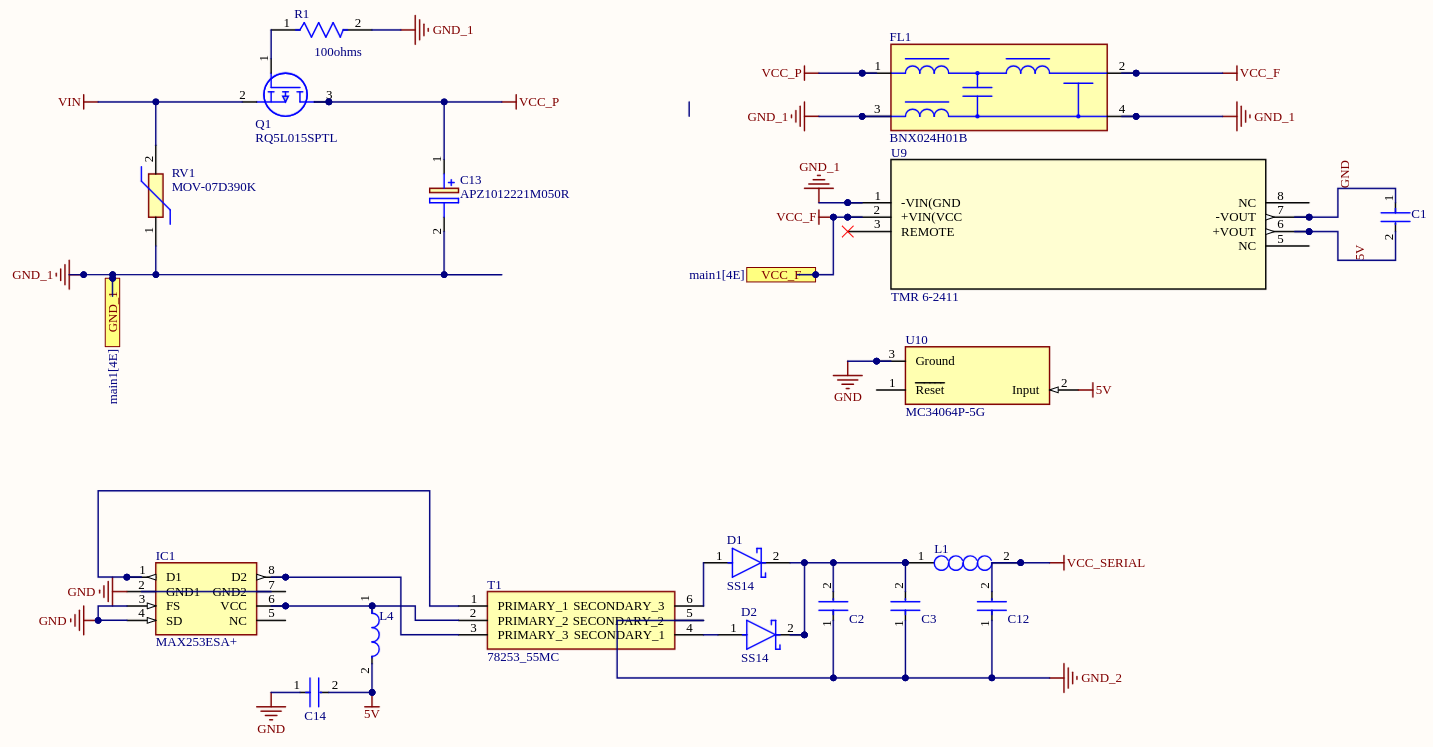
\includegraphics[width=\linewidth]{images/circuito01.png}

            \textbf{Fonte:} Autoria Própria
            \label{fig:circuito001}
        \end{figure}

        A placa de circuito impresso foi projetada com base no circuito apresentado anteriormente, resultando nos esquemáticos subsequentes. Esses diagramas, disponíveis na Figura\autoref{fig:pcbs}. delineiam a disposição dos componentes, as trilhas de conexão e a pinagem do microcontrolador, assegurando a integridade dos sinais e a interface eletrônica apropriada. As placas foram desenvolvidas no software especializado Altium e fabricadas pela empresa Wego Sistemas, conforme o procedimento adotado na versão anterior.

        \begin{figure}[H]
            \centering
            \caption{Placas de Circuito Impresso}

            \subfloat[Placa Modificada (Desenho)]{
                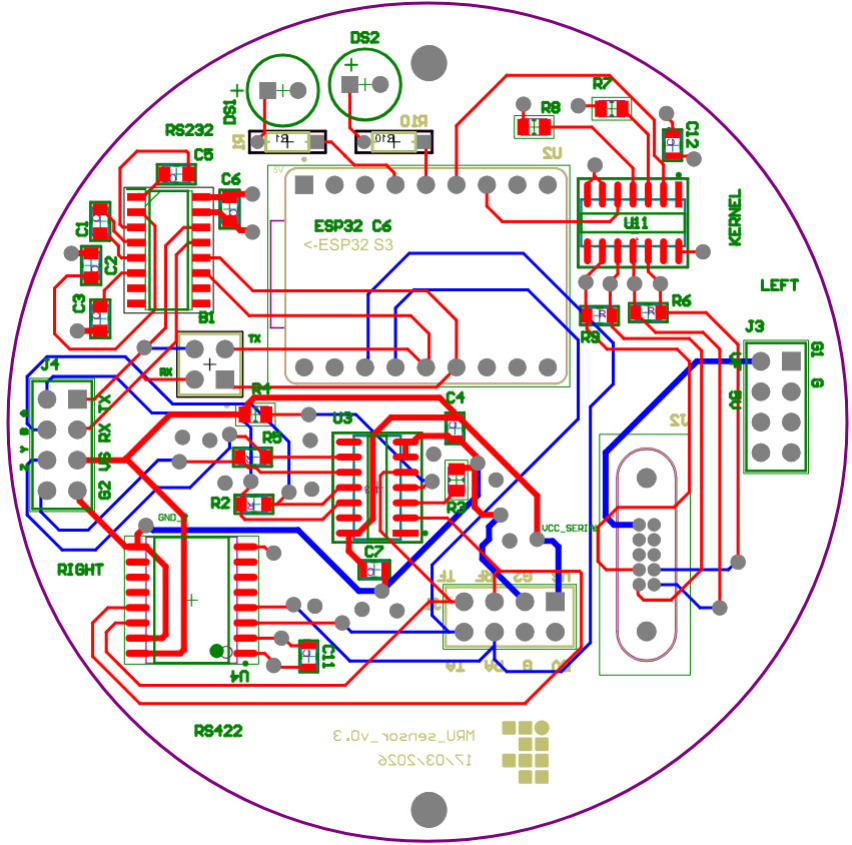
\includegraphics[height=5cm]{images/pcb1.png}
            }\hfill
            \subfloat[Placa Inferior]{
                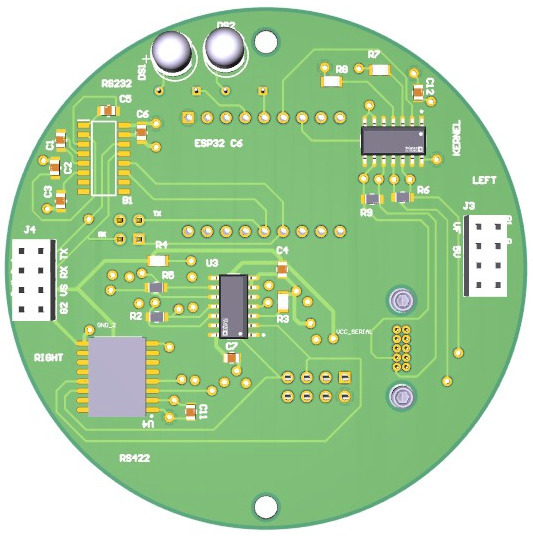
\includegraphics[height=5cm]{images/pcb2.png}
            }\hfill
            \subfloat[Placa Superior]{
                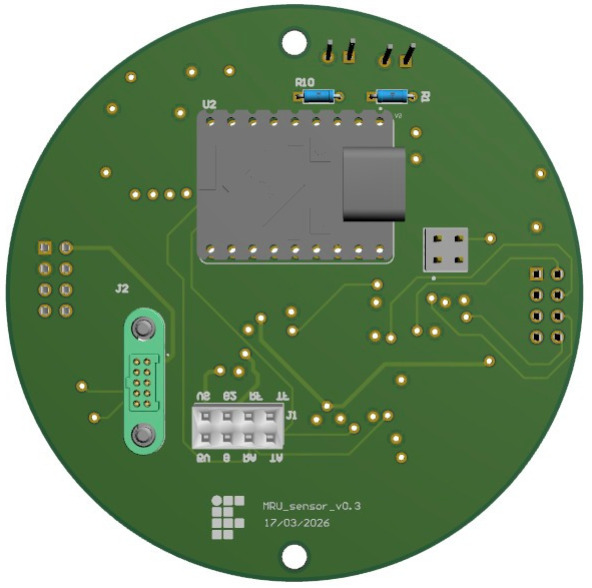
\includegraphics[height=5cm]{images/pcb3.png}
            }

            \textbf{Fonte:} Autoria Própria
            \label{fig:pcbs}
        \end{figure}

        A esquematização em três dimensões das placas aparece na Figura\autoref{fig:pcbs_3d} para permitir uma melhor visualização e ajustes finos como o formato circular comum em dispositivos semelhantes. Esse formato é estável e ajuda na adaptação do compartimento que envolve o dispositivo em três dimensões. 

        \begin{figure}[H]
            \centering
            \caption{Placas de Circuito Impresso 3D}

            \subfloat[]{
                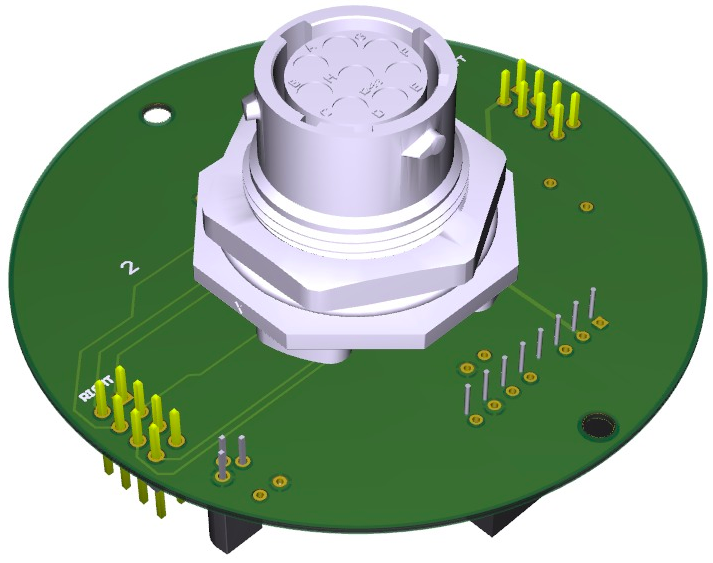
\includegraphics[height=3.5cm]{images/pcb_3d_1.png}
            }\hfill
            \subfloat[]{
                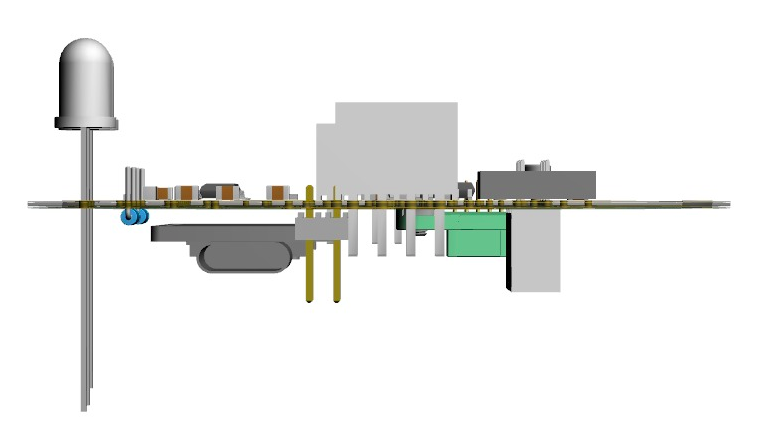
\includegraphics[height=3.5cm]{images/pcb_3d_2.png}
            }\hfill
            \subfloat[]{
                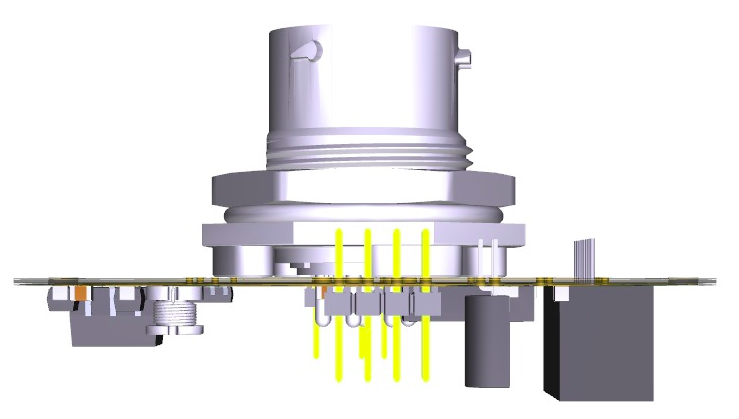
\includegraphics[height=3cm]{images/pcb_3d_3.png}
            }

            \textbf{Fonte:} Autoria Própria
            \label{fig:leticia}
        \end{figure}
        
        A placa física final pode ser visualizada na Figura\autoref{fig:leticia}. Ela foi montada e testada de modo a assegurar proteção contra intempéries e vibrações mecânicas severas, em conformidade com normas de robustez aplicáveis a ambientes offshore. 

        \begin{figure}[H]
            \centering
            \caption{Placa Fisica Montada}
            
            \subfloat[]{
                \frame{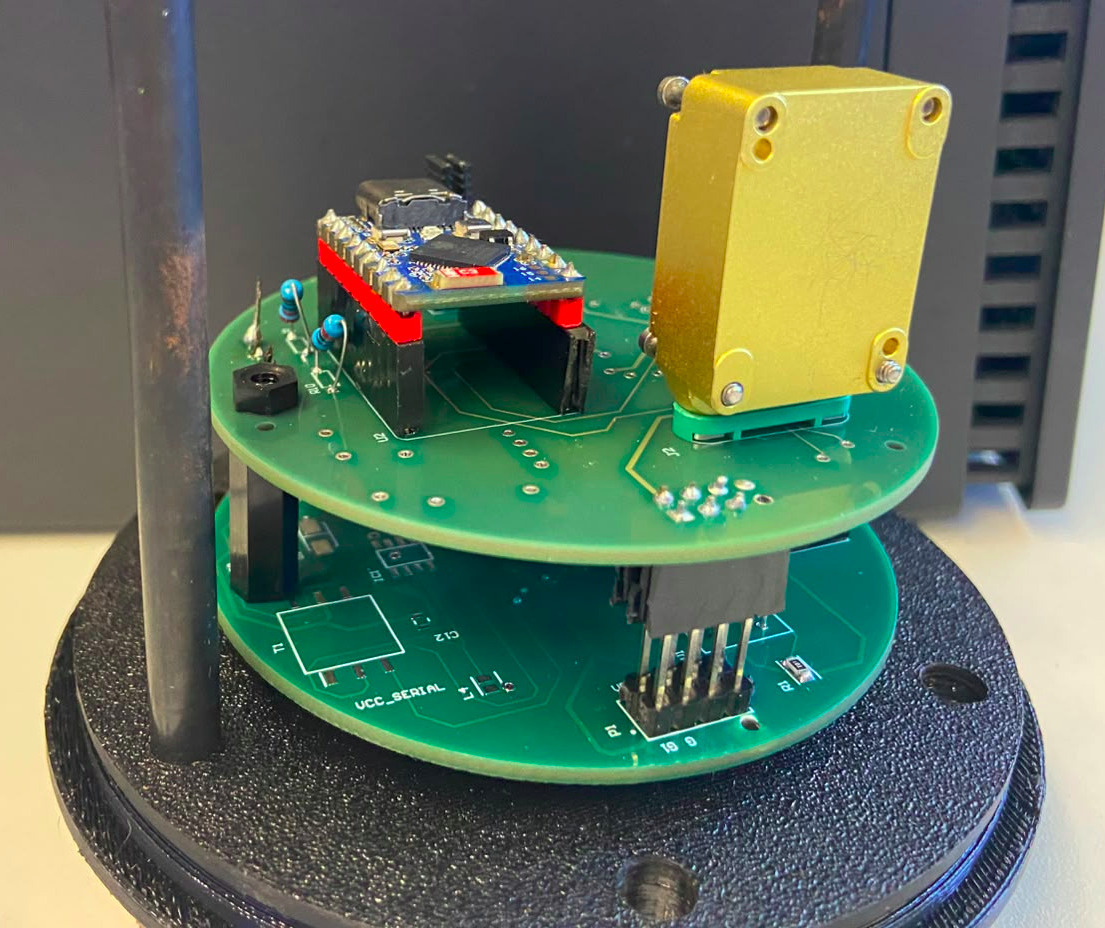
\includegraphics[height=5.5cm]{images/leticia1.png}}
            }
            \subfloat[]{
                \frame{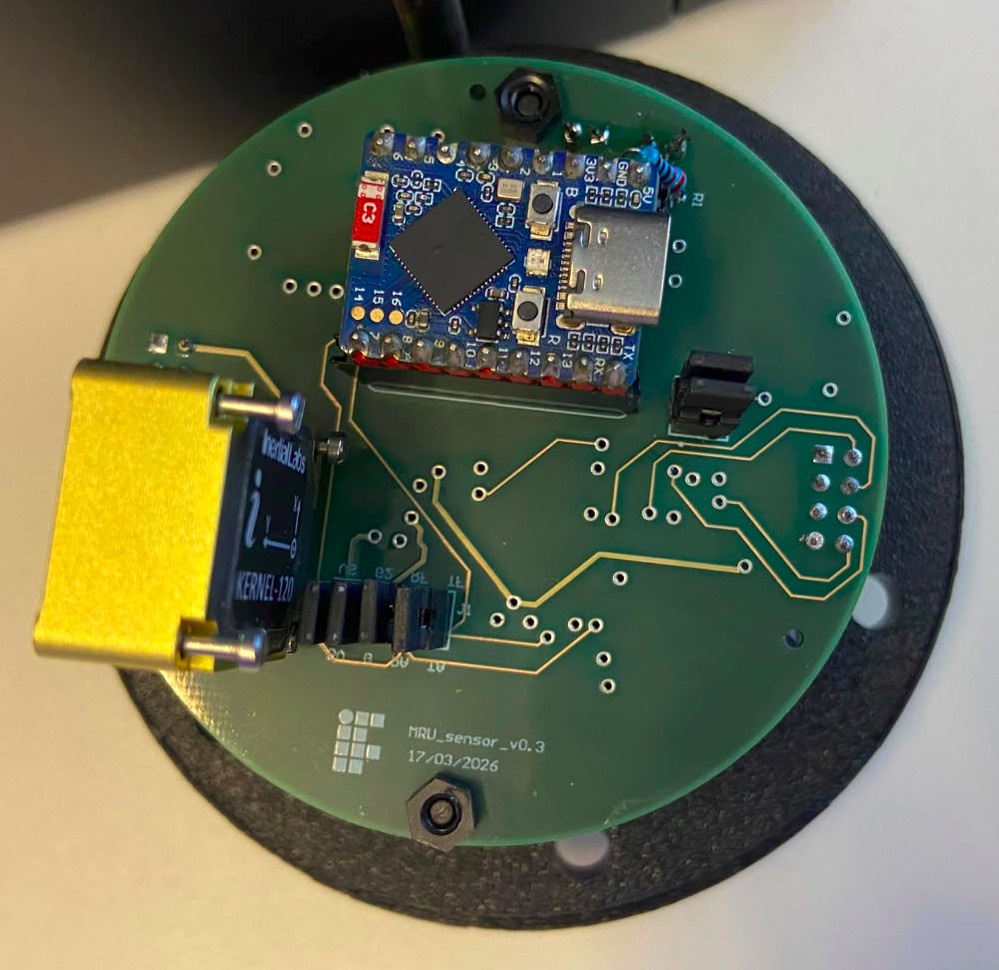
\includegraphics[height=5.5cm]{images/leticia2.png}}
            }
            \subfloat[]{
                \frame{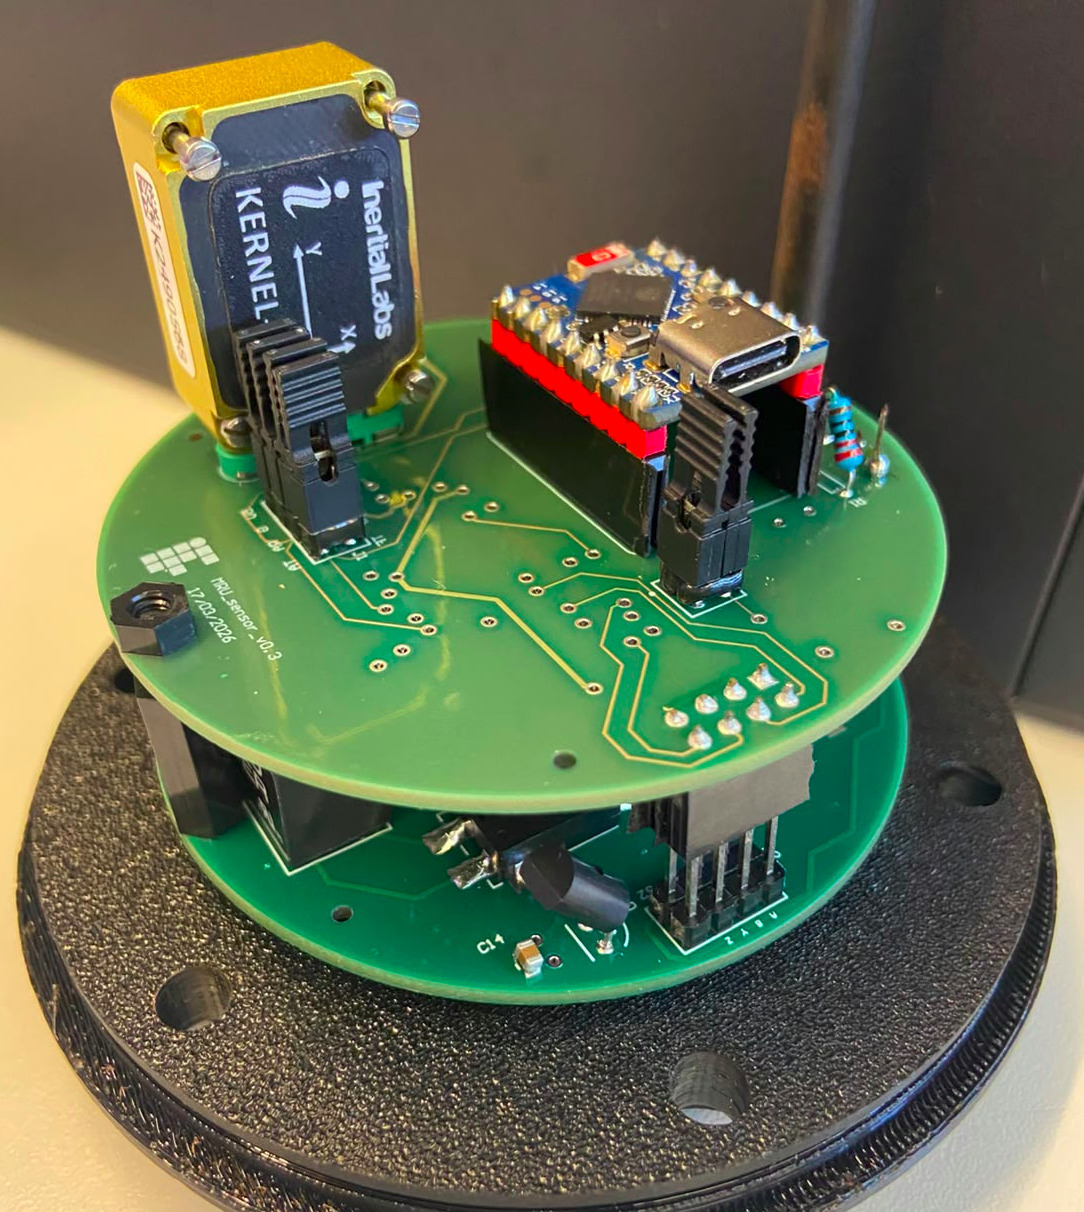
\includegraphics[height=5.5cm]{images/leticia3.png}}
            }
            
            \label{fig:graf_stew}
            \textbf{Fonte:} Autoria Própria
        \end{figure}
        
        Dentre as novas funcionalidades, foram incorporados LEDs para indicação visual de status: um informa o funcionamento dos componentes do sistema pela frequência com que o LED acende e apaga, e o outro refere-se à comunicação de dados, cuja frequência corresponde à velocidade de transmissão.

        \subsection{Desenhos Técnicos das Embalagens}
            Semelhante aos circuitos as embalagens também receberam modificações simples e evoluíram para uma segunda versão mostrada na \autoref{fig:desenho}. A embalagem serve para guardar de forma segura todos os componentes em um compartimento dedicado com proteção contra umidade e impactos mecânicos em condições expostas. 
            
            \begin{figure}[H]
                \centering
                \caption{Desenho Técnico das Embalagens}
                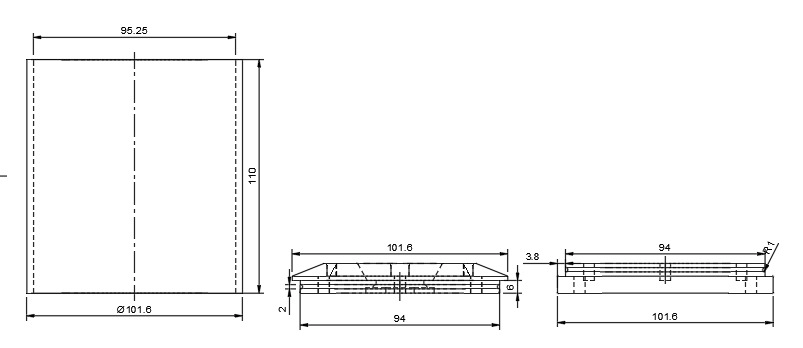
\includegraphics[width=.8\linewidth]{images/desenho_tecnico.png}
    
                \textbf{Fonte:} Autoria Própria
                \label{fig:desenho}
            \end{figure}
            
            A figura subsequente apresenta a embalagem definitiva com o sistema embarcado devidamente instalado. Os eixos cartesianos $X$, $Y$ e $Z$, correspondentes às três dimensões de movimento, estão perfeitamente alinhados com a caixa, acompanhados das indicações necessárias para facilitar o alinhamento durante a instalação. Dessa forma, concretiza-se o dispositivo final do projeto, resta apenas a validação qualitativa, a ser apresentada nas seções subsequentes.

            \begin{figure}[H]
                \centering
                \caption{Placa Fisica Montada}
                
                \subfloat[Peças Prontas]{
                    \frame{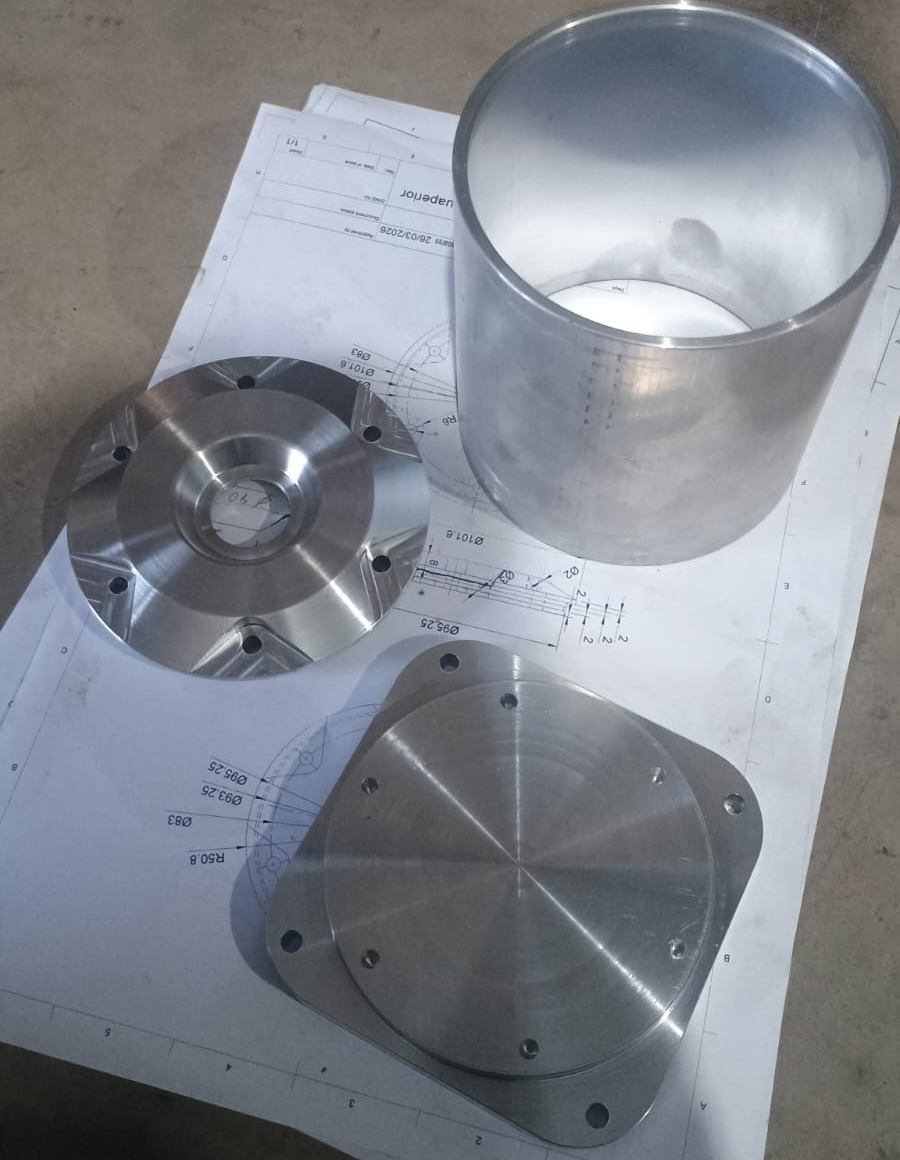
\includegraphics[height=8cm]{images/metal1.png}}
                }\hspace{1cm}
                \subfloat[Montagem]{
                    \frame{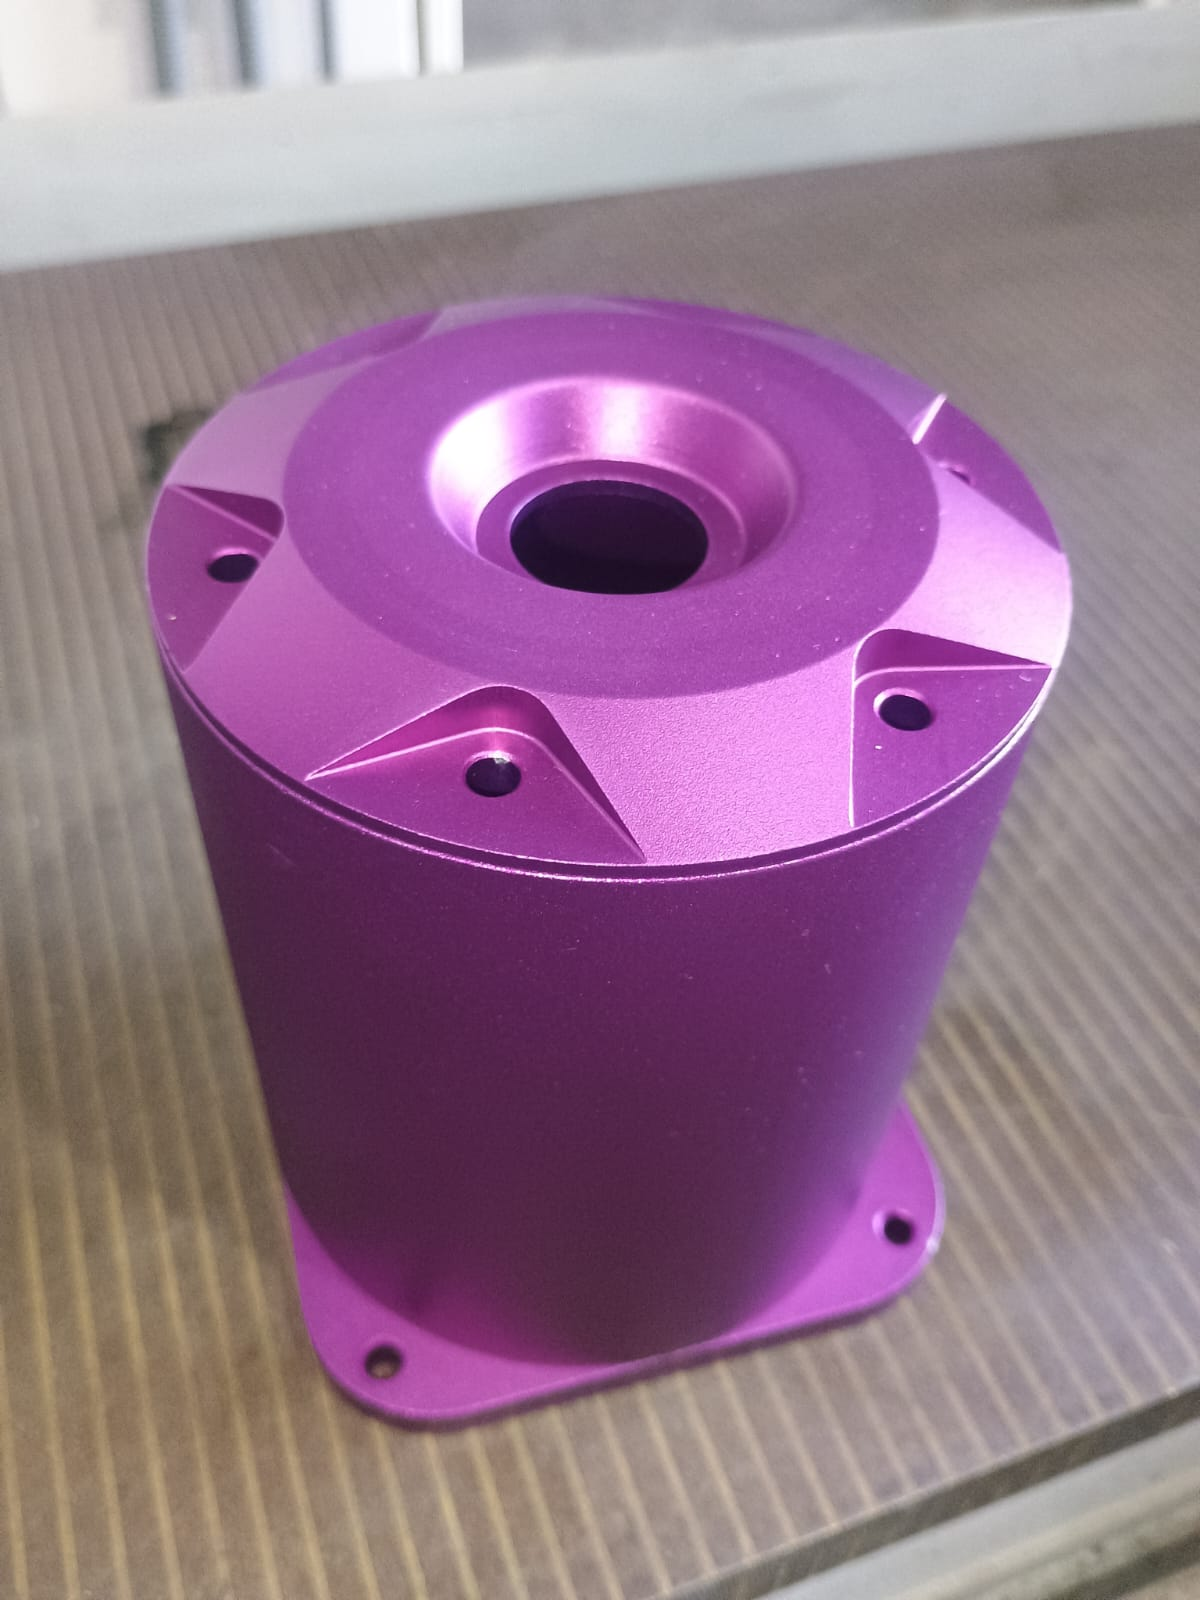
\includegraphics[height=8cm]{images/metal2.png}}
                }
                
                \label{fig:graf_stew}
                \textbf{Fonte:} Autoria Própria
            \end{figure}
            

            Além disso foram realizadas avaliações térmicas para garantir que a dissipação de calor dos componentes eletrônicos permaneça dentro dos limites operacionais mesmo sob sol direto em plataformas offshore. O sensor de temperatura está embutido no próprio Kernel, que exibe aquecimento inerente (como típico de sensores de movimento) e requer controle térmico robusto para evitar o superaquecimento do sensor e dos demais componentes. Este sensor constitui o elemento mais crítico de monitoramento, uma vez que gera a maior dissipação térmica. Esse parâmetro foi monitorado continuamente em campo por 12 horas, com o gráfico de temperatura apresentado na figura subsequente.

            \begin{figure}[H]
                \centering
                \caption{Monitoramento da Temperatura Dentro da Embalagem}
                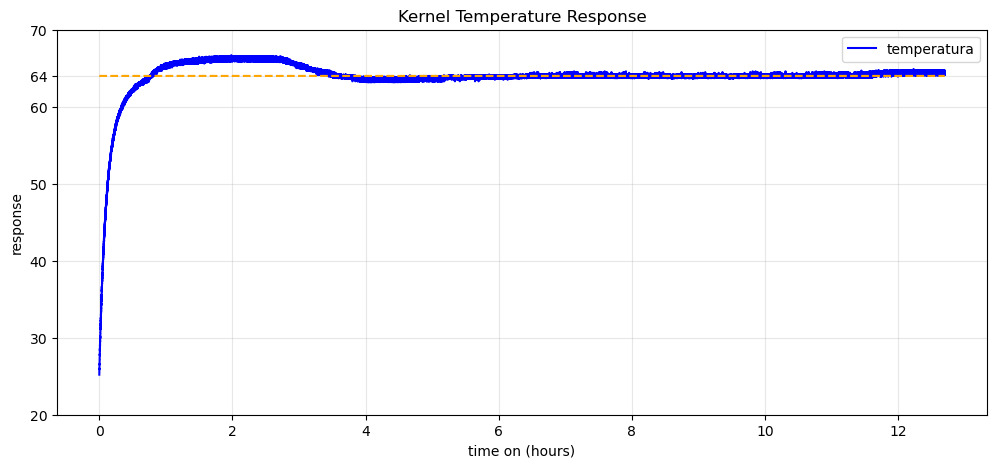
\includegraphics[width=.8\linewidth]{images/temperatura.png}
    
                \textbf{Fonte:} Autoria Própria
                \label{fig:circuito01}
            \end{figure}

            Observa-se que, ao ativar o sistema, a temperatura inicia no valor ambiente, conforme esperado. À medida que o sensor aquece pela dissipação de calor, a temperatura sobe de forma exponencial e a curva térmica estabiliza em um patamar operacional constante em torno de 64 graus Celsius. Esse comportamento mostra que a dissipação térmica é controlada de modo adequado, sem comprometer a integridade do hardware nem a precisão das leituras inerciais em uso prolongado. A temperatura, embora pareça elevada, fica dentro da faixa operacional de todos os componentes integrados. A temperatura, apesar de subir, não atingiu nível crítico, o que validou a eficácia do projeto térmico e a capacidade da embalagem de dissipar o calor gerado pelos componentes internos.

    \subsection{Relatório Final}
        O Relatório Final do projeto representa a consolidação abrangente de todas as etapas desenvolvidas, unindo as cinco macroentregas anteriores com o relatório detalhado de calibração e os resultados completos dos testes realizados. Essa estrutura foi adotada para oferecer uma visão integrada do progresso do projeto, facilitando a rastreabilidade de todos os artefatos gerados, desde os desenhos técnicos e manuais até os códigos-fonte e validações experimentais, além de documentar de forma clara os dados brutos, gráficos analíticos e métricas de desempenho obtidos nos experimentos estáticos e dinâmicos. Adicionalmente, esta seção consolida a análise da confiabilidade metrológica dos sistemas inerciais sob perfis dinâmicos, garantindo a rastreabilidade dos parâmetros de estabilização e atestando a maturidade do protótipo para implantação em ambientes marítimos reais.

    \subsection{Patentes, Desenhos Industriais e Registro de Softwares}
        Esta seção destina-se ao registro da documentação referente à proteção da propriedade intelectual gerada pelo projeto. Os dois programas protegidos correspondem ao software de monitoramento das variáveis, também designado como HMS, e ao firmware embarcado no microcontrolador, desenvolvido na linguagem de programação C++. A seguir, apresentam-se os dados técnicos para o registro do software elaborado no âmbito do projeto PIFF-2411.0049:

\begin{center}
    \centering\footnotesize
    {\renewcommand{\arraystretch}{1.2}
    \begin{longtable}{|c|c|c|c|}
        \caption{Descrição e Códigos Hash dos Softwares} \label{tab:softwares}\\
        \hline
            \fcol{.20}{\textbf{Título do Software}} & 
            \col{.35}{\textbf{Descrição}} & 
            \col{.20}{\textbf{Linguagem de Programação}} & 
            \col{.25}{\textbf{Código Hash}} \\
        \hline 
            \fcol{.20}{SMH-Interface} & 
            \col{.35}{Interface web para visualização de telemetria, alertas de segurança e gestão de relatórios offshore.} & 
            \col{.20}{Javascript/Rust} & 
            \col{.25}{9b253ca6\allowbreak 6fdc2dff\allowbreak 39761d23\allowbreak c1aa9be8\allowbreak d01b3ec0\allowbreak 4c2bf38a\allowbreak 3209effe\allowbreak b8a563a} \\
        \hline
            \fcol{.20}{\textit{Firmware do Dispositivo de Referência de Monitoramento dos Movimentos (DRMM)}} & 
            \col{.35}{Sistema embarcado para aquisição e processamento de dados inerciais em tempo real nos helidecks.} & 
            \col{.20}{C++} & 
            \col{.25}{30b8e8fa\allowbreak b580bd8d\allowbreak dfa0cd71\allowbreak a8fcb0bd\allowbreak 33c084ea\allowbreak 6d6c8ee2\allowbreak c2758a33\allowbreak 426dc803} \\
        \hline
    \end{longtable}
    }

    \normalsize
    \textbf{Fonte:} Autor
\end{center}

        A documentação de propriedade intelectual registrada, com os hashes dos softwares SMH-Interface e Firmware do Dispositivo de Referência de Monitoramento dos Movimentos fornecidos na tabela acima, protege as inovações do projeto contra uso indevido, formalizando os direitos sobre os desenvolvimentos em interface web e sistema embarcado.

\section{Desenvolvimento}
    Com base na metodologia desenvolvida para o projeto, a seguir será descrita a implementação de cada subetapa do processo, abordando a usabilidade do dispositivo, sua calibração e o processo de validação. Fotografias foram anexadas para ilustrar o desenvolvimento global dos procedimentos.

    \subsection{Sistema Embarcado}
        A versão definitiva do firmware embarcado no IMU foi disponibilizada, incorporando o sensor Kernel na placa em conjunto com o microcontrolador do sistema. O desenvolvimento da programação do dispositivo ocorreu na IDE do Arduino, com estrutura modular para cada sensor e periférico, resultando em um programa principal unificado. Ao longo dos meses, o programa recebeu atualizações periódicas que incorporaram novas funcionalidades, como transmissão de dados via Protobuf ou serial, integração de protocolo otimizado, configuração de parâmetros operacionais e sistema de tratamento de erros. Essas atualizações garantiram a robustez do sistema perante falhas em componentes.

        \begin{figure}[H]
            \centering
            \caption{Imagem Dimensional do IMU}
            \frame{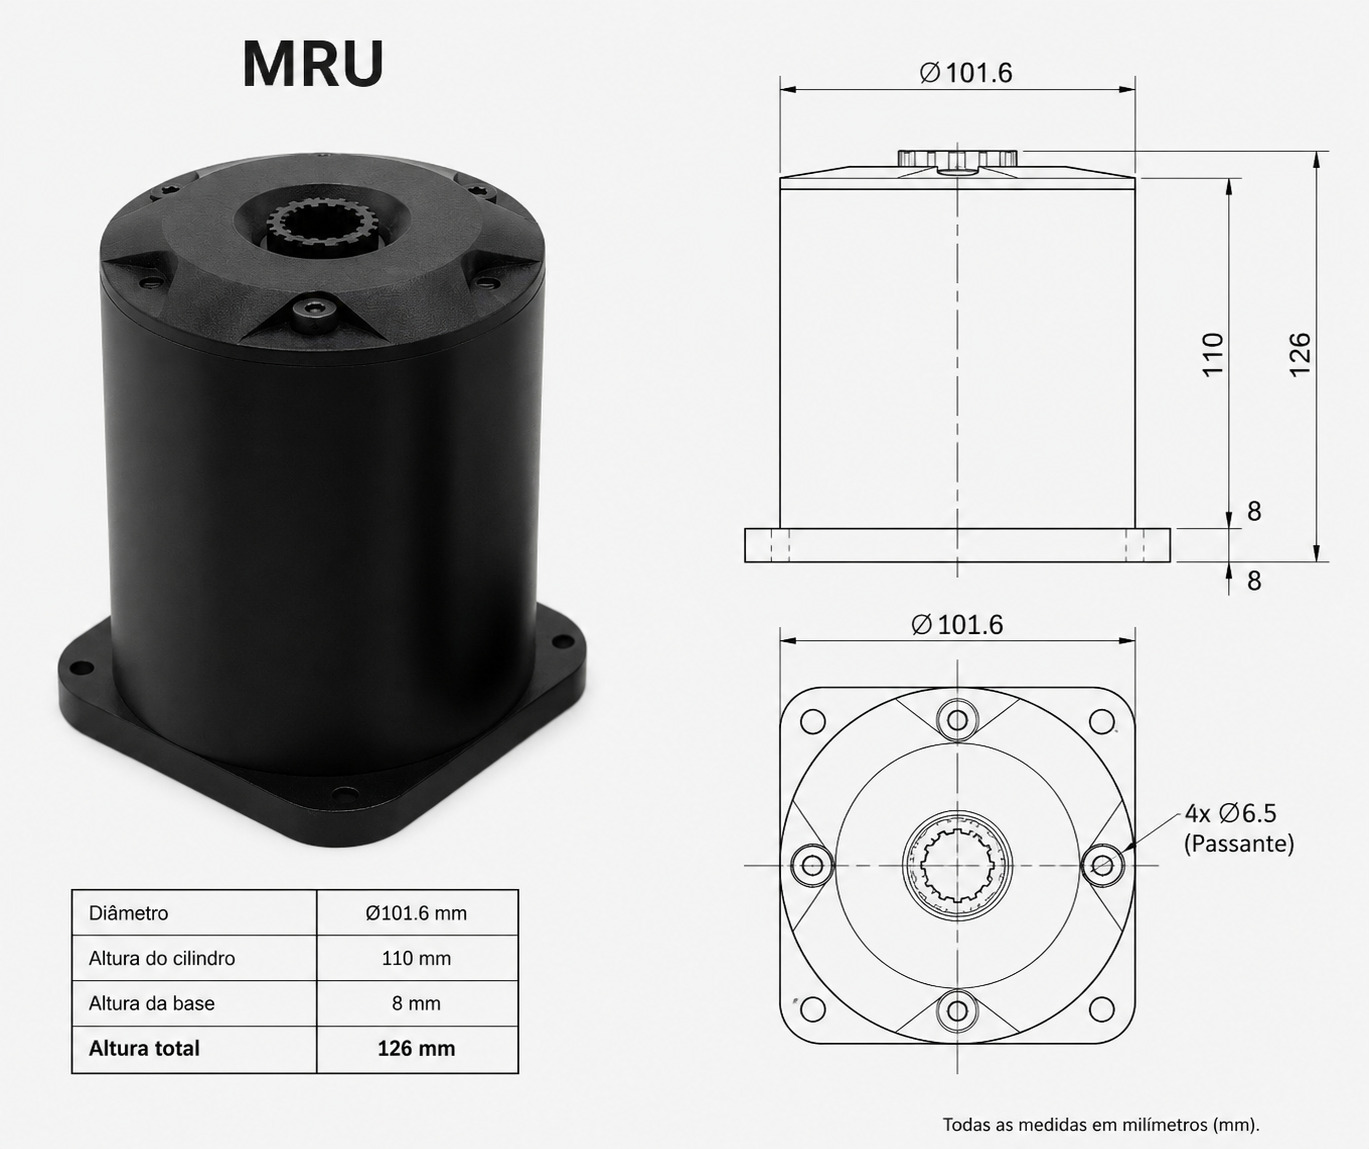
\includegraphics[height=10cm]{images/mru.png}}
            
            \textbf{Fonte:} Autoria Própria
            \label{fig:circuito01}
        \end{figure}

        A figura subsequente mostra um esquemático comercial desenvolvido para o manual de instalação de forma a orientar e apresentar o dispositivo com suas ligações elétricas para configuração, alimentação e extração de dados via protocolo RS232 e RS422.

        \begin{figure}[H]
            \centering
            \caption{Circuito do Sistema Embarcado}
            \subfloat[Compartimento]{
                \frame{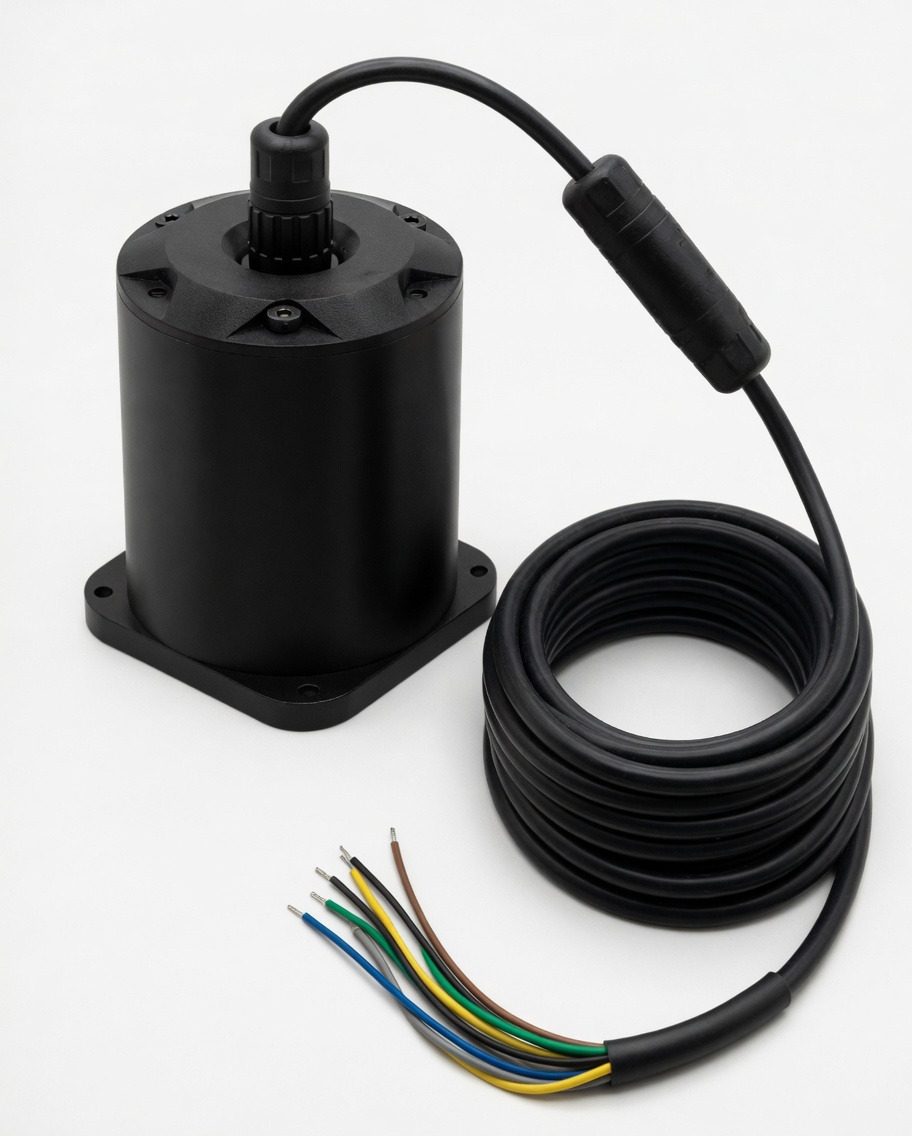
\includegraphics[height=10cm]{images/comercial1.png}}
            }\hfill
            \subfloat[Ligações Elétricas]{
                \frame{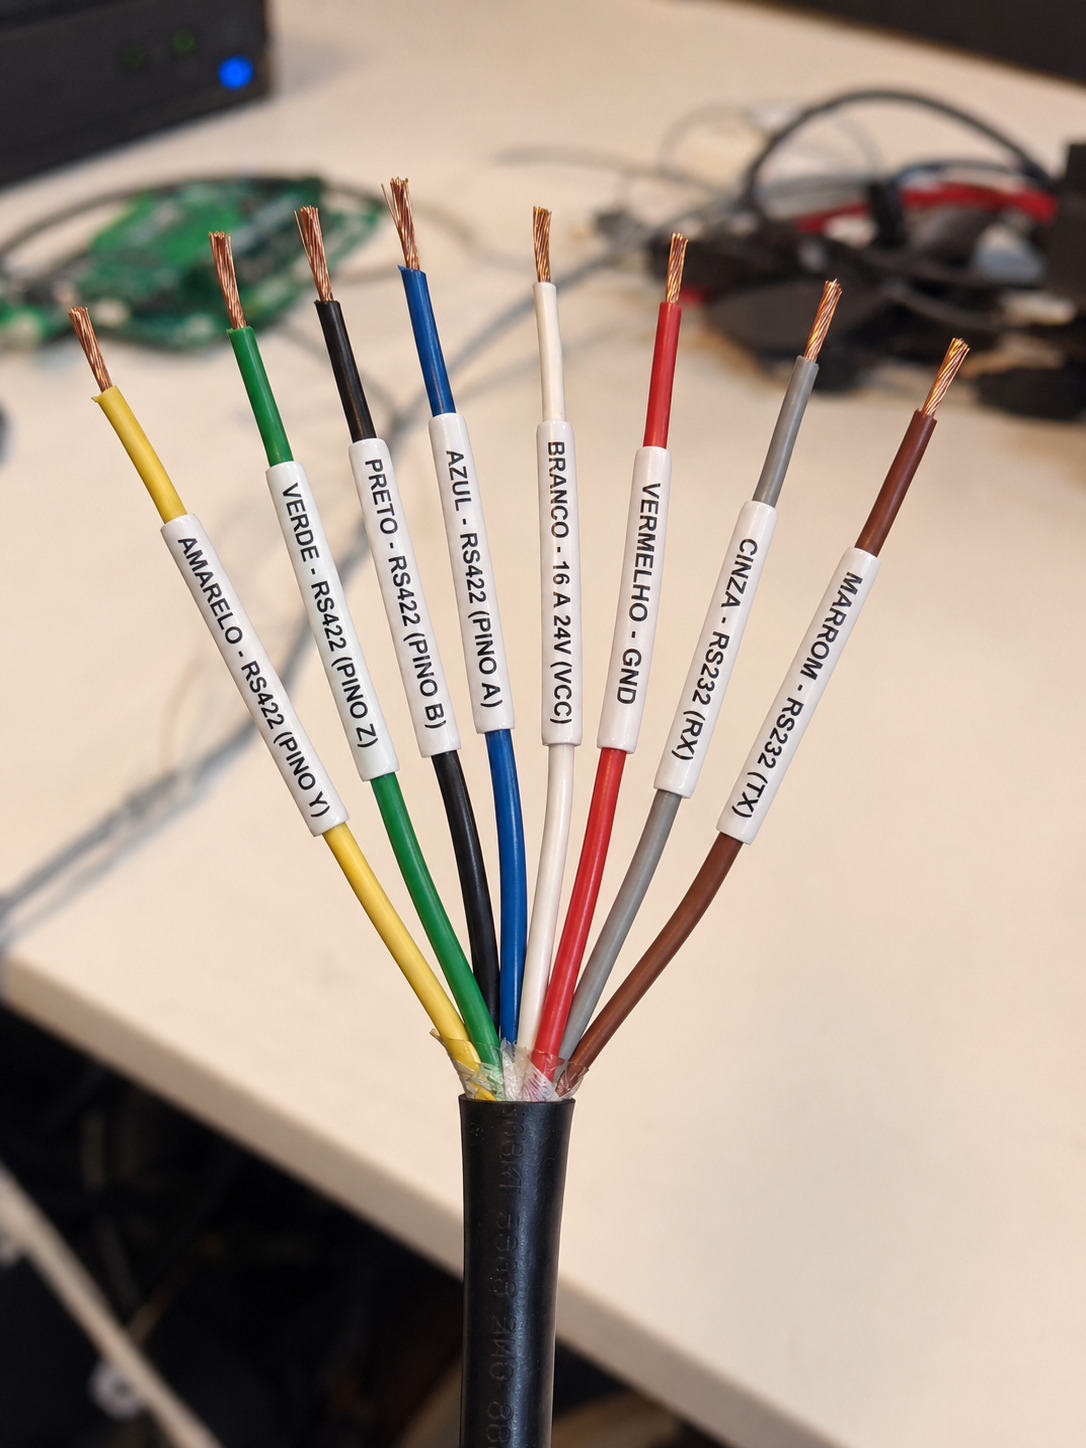
\includegraphics[height=10cm]{images/comercial2.png}}
            }

            \textbf{Fonte:} Autoria Própria
            \label{fig:circuito01}
        \end{figure}
        
        As grandezas medidas são transmitidas tanto no formato JSON quanto em formato binário otimizado, conforme o protocolo NMEA, conferindo flexibilidade à integração com diversos sistemas de gestão e visualização, além de otimizar a transmissão de dados. A orientação do sensor é apresentada na Figura\autoref{fig:graf_stew}.
        
        \begin{figure}[H]
            \centering
            \caption{Orientação Utilizada}
            \subfloat[Orientação Cartesiana 3D]{
                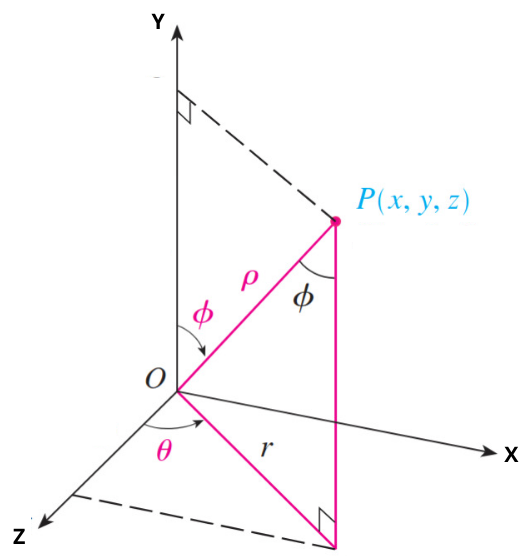
\includegraphics[height=5.5cm]{images/graf3d.png}
            }
            \subfloat[Orientação do Sensor Kernel]{
                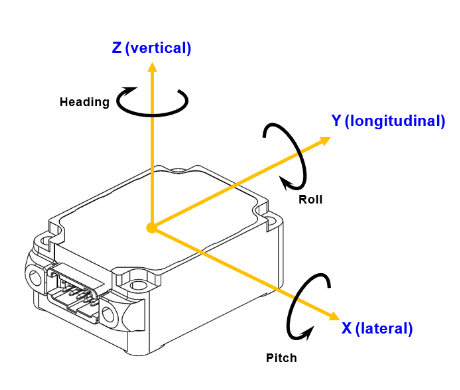
\includegraphics[height=5.5cm]{images/kernel2.png}
            }
            \subfloat[Orientação do Sensor Kernel]{
                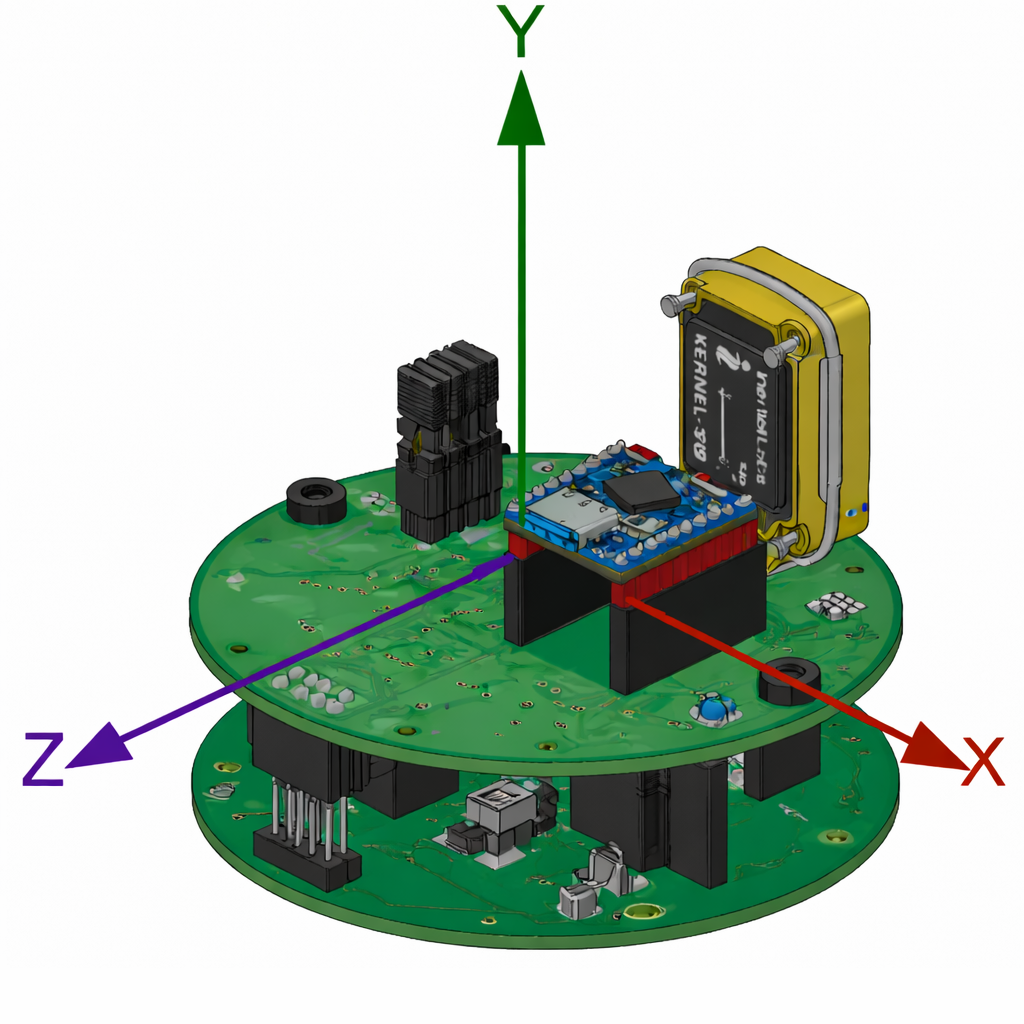
\includegraphics[height=5.5cm]{images/kernel3.png}
            }
            
            \label{fig:graf_stew}
            \textbf{Fonte:} Autoria Própria
        \end{figure}

        A taxa de transmissão das variáveis é de 100 Hz, admitindo ajustes via configuração; no protocolo, enviam-se as variáveis pitch, roll e yaw, enquanto no JSON incluem-se as acelerações lineares e velocidades angulares captadas pelo sensor. 

    \subsection{Software de Monitoramento}
        Em paralelo, o software de supervisão foi portado para uma aplicação desktop completa desenvolvida em Tauri, integrando tecnologias JavaScript com React e Rust. Isso visa otimizar o desempenho e a interface do usuário, conferindo uma experiência de monitoramento mais eficiente, interativa e graficamente representativa. A \autoref{fig:hms} ilustra a interface funcional do software de monitoramento.

        \begin{figure}[H]
            \centering
            \caption{Monitoramento pelo HMS}
            \frame{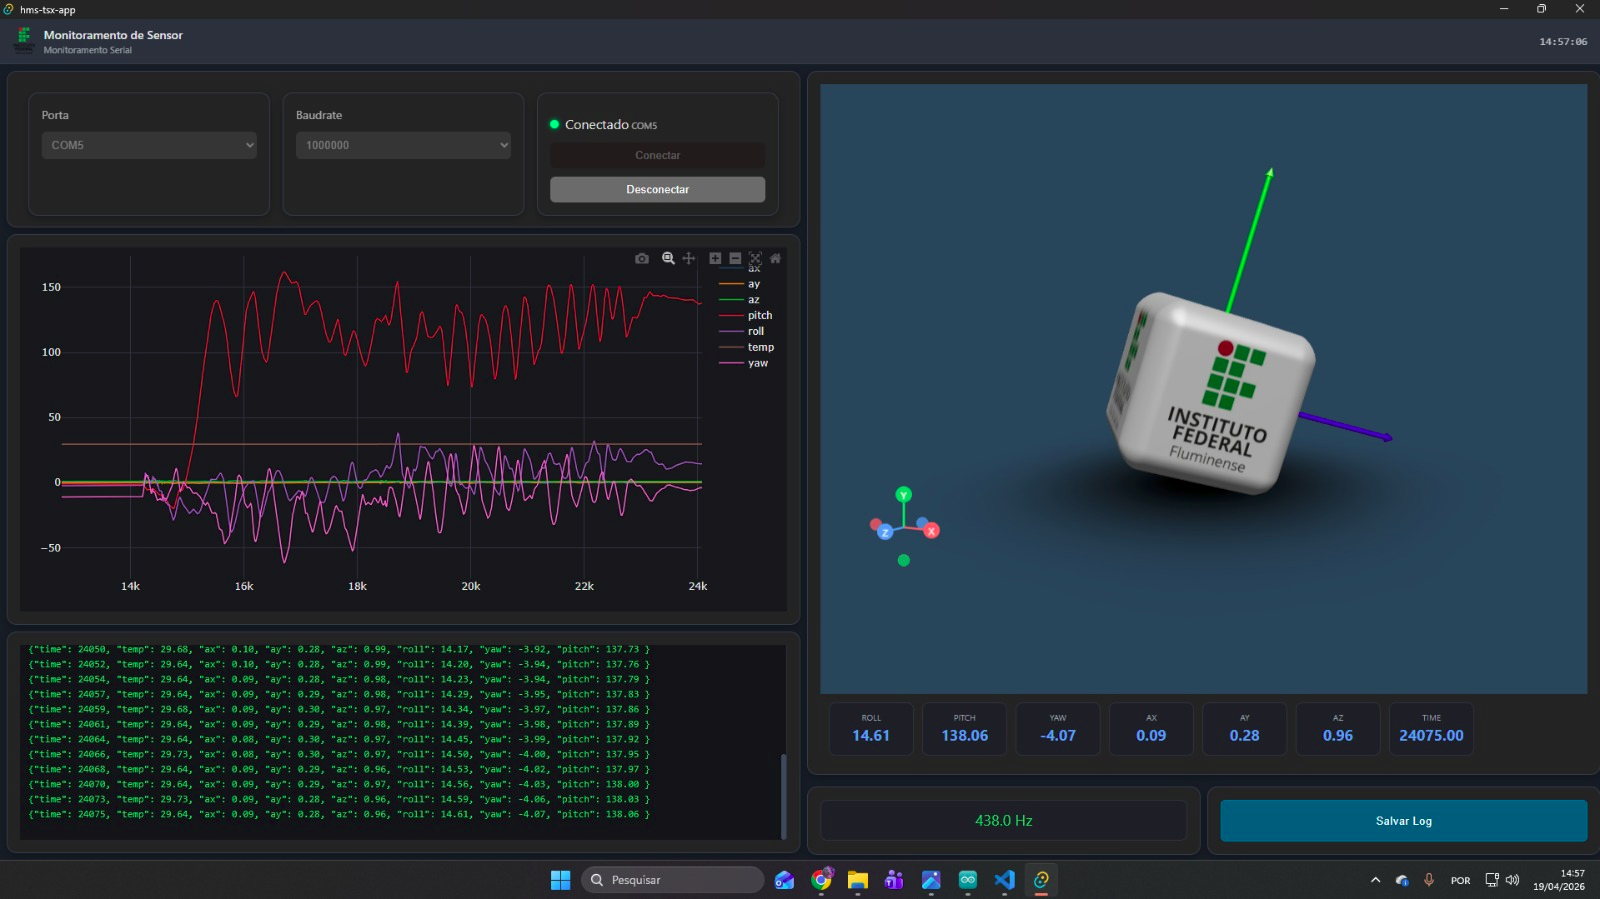
\includegraphics[width=\linewidth]{images/hms.png}}
        
            \textbf{Fonte:} Autoria Própria
            \label{fig:hms}
        \end{figure}

        O software possibilita monitoramento dos dados extraídos em tempo real, e que podem ser baixados em formatos JSON ou CSV, viabilizando análises posteriores específicas. Essa funcionalidade revela-se essencial para a comparação com outro dispositivo de monitoramento, o qual será utilizado na validação do protótipo desenvolvido. A figura subsequente apresenta imagens do dispositivo de monitoramento implementado e funcional, acompanhadas da respectiva interface gráfica.

        \begin{figure}[H]
            \centering
            \caption{HMS Rodando com Testes do Pêndulo}
            \frame{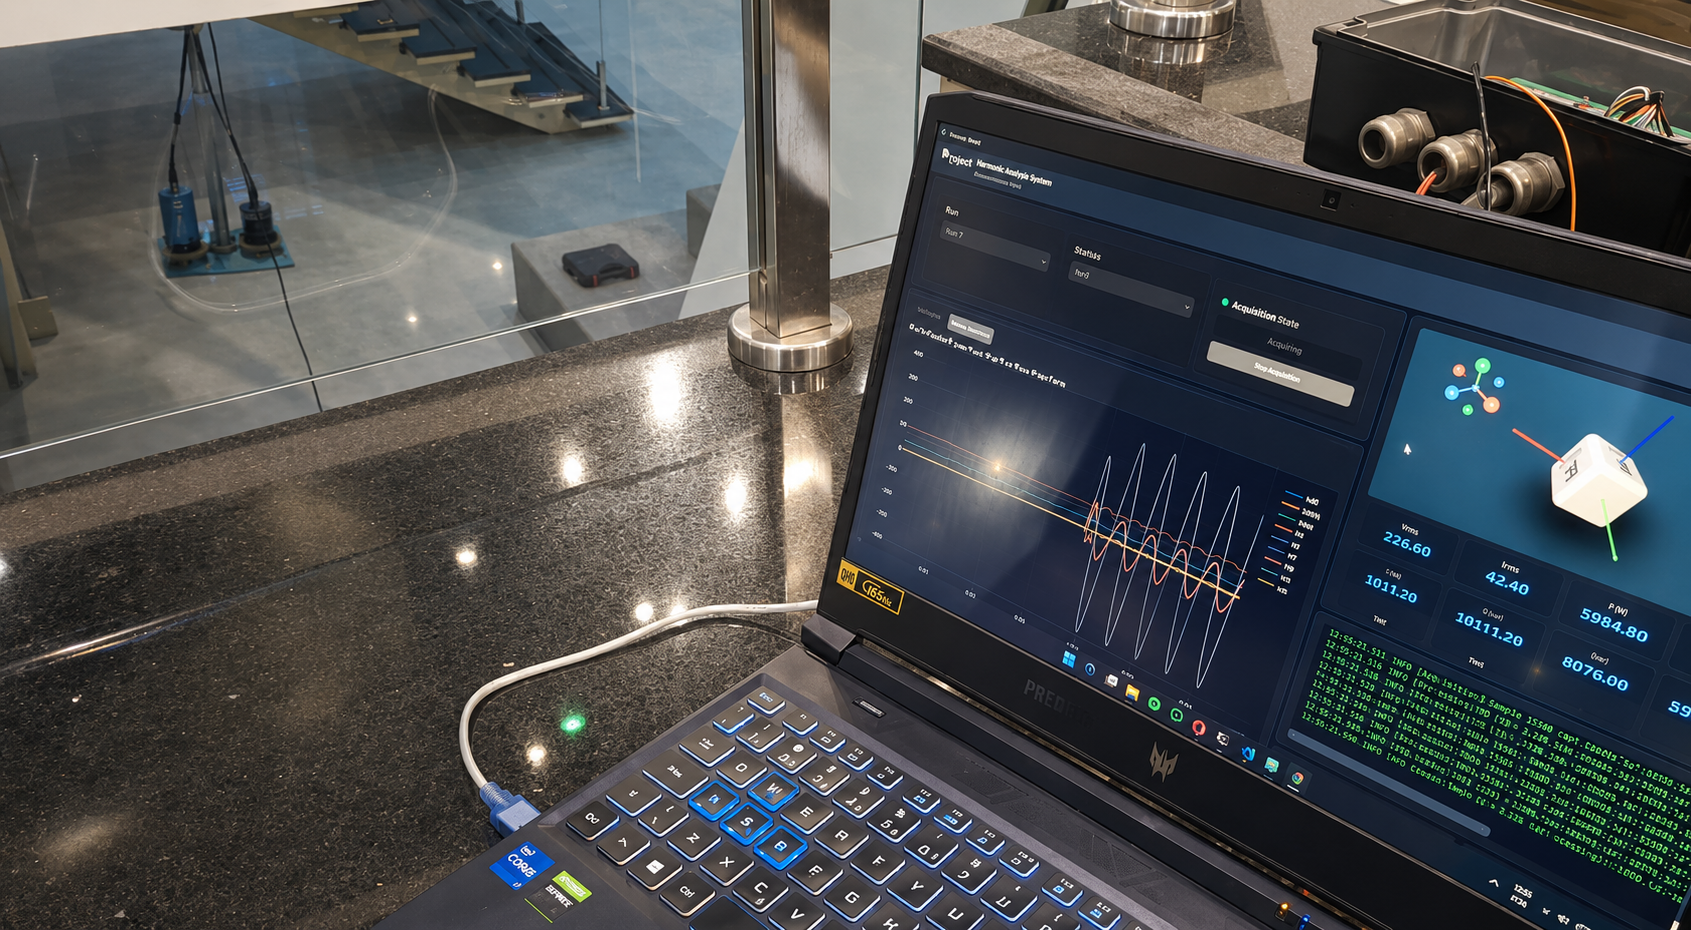
\includegraphics[width=\linewidth]{images/ChatGPT Image Jun 1, 2026, 01_39_17 PM.png}}
        
            \textbf{Fonte:} Autoria Própria
            \label{fig:hms2}
        \end{figure}

         Para a transmissão de dados utilizada na comunicação RS422, de forma a atender às exigências do software de monitoramento quanto ao formato dos dados do DRMM e garantir o alinhamento com as normativas de mercado, optou-se pela implementação do protocolo NMEA. Baseado principalmente no padrão de comunicação serial assíncrona RS-422, este protocolo utiliza o padrão ASCII para codificar as informações em sentenças legíveis, divididas em campos delimitados com funções específicas de identificação, dados e checagem. 

    \subsection{HMS}
        O desenvolvimento do aplicativo desktop de monitoramento foi direcionado para ter um foco comercial e atender às expectativas atuais do setor. As telas do programa foram estruturadas com base em soluções já consolidadas, como o sistema dedicado da empresa Kongsberg. Além disso, o software foi projetado para indicar as variáveis de movimento Pitch, Roll e Yaw de maneira contínua e puramente numérica. Contudo, o foco central dessa abordagem técnica é simplificar a operação diária. Logo, o formato adotado garante aos usuários uma facilidade significativamente maior na visualização dos dados.
        
        \begin{figure}[H]
            \centering
            \caption{HMS Comercial do Sistema}
            \subfloat[Modelo Kongsberg]{
                \frame{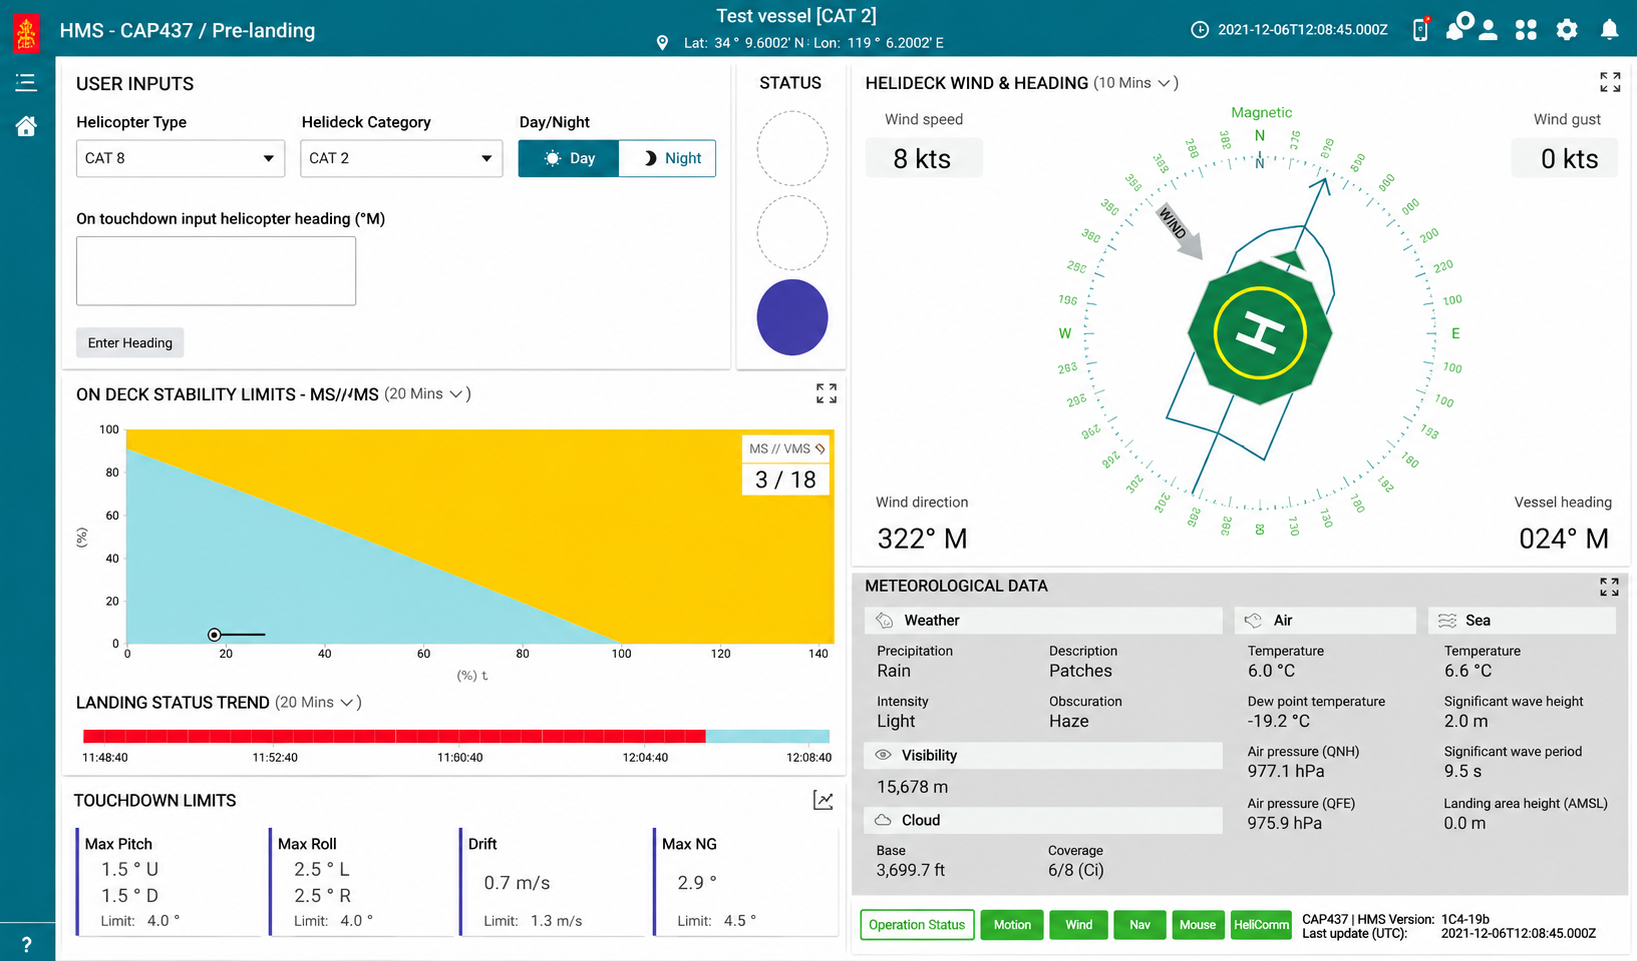
\includegraphics[height=4.6cm]{images/hms1.png}}
            }\hfill
            \subfloat[Modelo Measure]{
                \frame{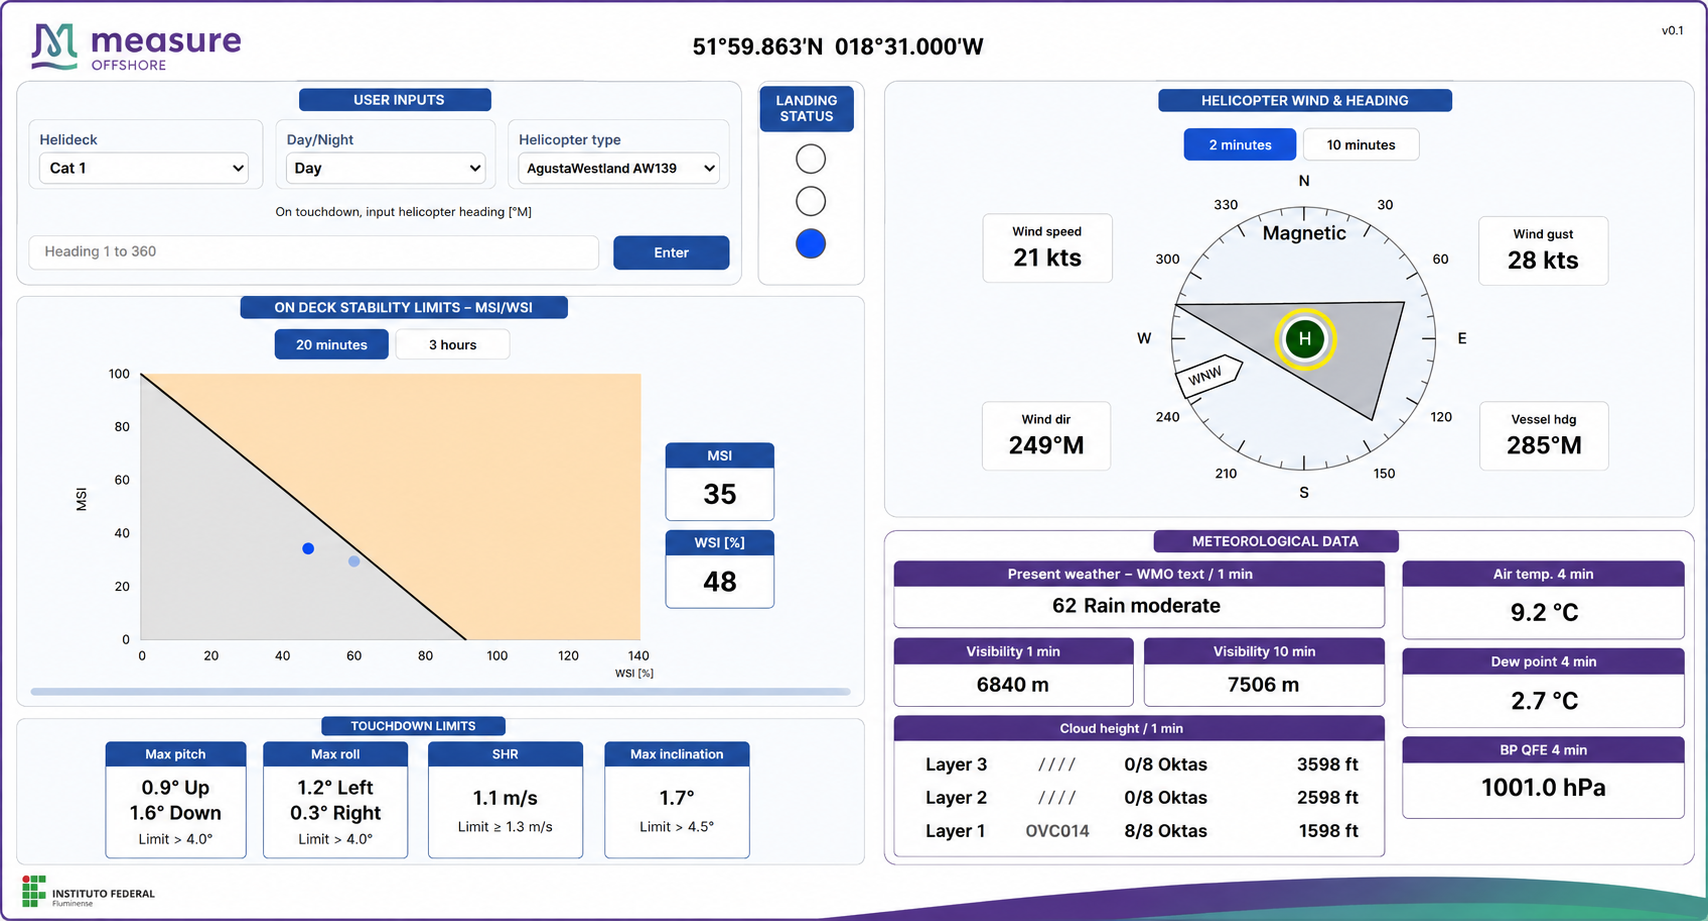
\includegraphics[height=4.6cm]{images/hms2.png}}
            }

            \textbf{Fonte:} Autoria Própria
            \label{fig:circuito01}
        \end{figure}

        As outras variáveis gráficas e numéricas estão disponíveis no sistema apenas de forma simbólica. Isso ocorre porque somente as três informações de orientação têm origem direta no MRU. Além disso, os demais dados são provenientes de sensores externos que não integram o escopo do projeto atual. Contudo, a aplicação atua como uma ferramenta indicativa totalmente escalável. Logo, o sistema poderá estabelecer comunicação com diversos equipamentos e sensores no futuro, o que permitirá o seu funcionamento integrado em uma estação sensorial embarcada.
        

    \subsection{Protocolo de Informação/Configuração}
    
    Para a comunicação RS232, que será utilizada primariamente para extração de informações do dispositivo e configuração do mesmo, o protocolo desenvolvido pela equipe estabelece o fluxo de intercâmbio de mensagens entre os dispositivos, operando com um baud rate configurável. A saída é um texto puro em formato ASCII, também funcionando para o envio e recebimento. Os eventos enviados e as respostas recebidas obedecem a seguinte estrutura:

    \begin{center}
        \begin{tabular}{|c|c|c|}
        \hline
             \phantom{aa} Início \phantom{aa}  & \phantom{aa}  Payload (dados) \phantom{aa}  &  \phantom{aa} Fim \phantom{aa}   \\
        \hline
             \texttt{\$} & \texttt{comando} & \texttt{!} \\
        \hline
        \end{tabular}
    \end{center}

    \begin{itemize}
        \item \texttt{\$} $\Rightarrow$ Delimitador de início de mensagem.
        \item \texttt{comando} $\Rightarrow$ A instrução ou dado a ser processado.
        \item \texttt{!} $\Rightarrow$ Delimitador de fim de mensagem.
    \end{itemize}

\begin{center}
    \centering\footnotesize
    {\renewcommand{\arraystretch}{1.2}
    \begin{longtable}{|c|c|c|}
        \caption{Protocolo de Comunicação}
        \label{tab:protocol}\\
        \hline
            \fcol{.27}{\textbf{Evento}} & 
            \col{.45}{\textbf{Descrição}} & 
            \col{.28}{\textbf{Resposta}} \\
        \hline
            \fcol{.27}{\cmd{stream\_start}} & 
            \col{.45}{Inicia a transmissão de dados de movimento no protocolo indicado} & 
            \col{.28}{Dados, podendo ser em JSON, Lista ou NMEA} \\
        \hline
            \fcol{.27}{\cmd{MICRS}} & 
            \col{.45}{Reinicia o dispositivo} & 
            \col{.28}{Vazio - Dispositivo Reiniciado} \\
        \hline
            \fcol{.27}{\cmd{stream\_stop}} & 
            \col{.45}{Interrompe a transmissão de dados de movimento no protocolo indicado} & 
            \col{.28}{Vazio (encerramento da transmissão)} \\
        \hline
            \fcol{.27}{\cmdi{ID}{baudrate}} & 
            \col{.45}{Retorna o baud rate atual configurado para o dispositivo} & 
            \col{.28}{Ex: \cmdi{ID}{baudrate} retorna \cmd{9600} } \\
        \hline
            \fcol{.27}{\cmdc{CF}{baudrate}{XXXXX}} & 
            \col{.45}{Configura o baud rate do dispositivo para o valor desejado} & 
            \col{.28}{Ex: \cmdc{CF}{baudrate}{115200} configura o baudrate para 115200} \\
        \hline
            \fcol{.27}{\cmdi{ID}{frequency}} & 
            \col{.45}{Retorna a frequência de amostragem atual configurada para o dispositivo} & 
            \col{.28}{Ex: \cmdi{ID}{frequency} retorna \cmd{50Hz}} \\
        \hline
            \fcol{.27}{\cmdc{CF}{frequency}{XXX}} & 
            \col{.45}{Configura a frequência de transmissão (ex: 10Hz, 50Hz, 100Hz) do dispositivo} & 
            \col{.28}{Ex: \cmdc{CF}{frequency}{100} configura a 100Hz} \\
        \hline
    \end{longtable}
    }

    \normalsize
    \textbf{Fonte:} Autor
\end{center}

    \noindent\obs os comandos de configuração só farão efeito após reiniciar o dispositivo com o comando \cmd{MICRS}   
       
    
    \subsection{Testes de Campo}
        Os testes de campo permitiram ajustar e modificar a metodologia de calibração de forma a aprimorar o sistema. A plataforma principal empregada foi o pêndulo, selecionado por sua simplicidade e eficiência linear com base nas equações físicas do sistema. A Figura\autoref{fig:pendulo} apresenta seu diagrama de corpo livre juntamente com uma esquematização 3D de uma instalação exemplar. Essa instalação serviu de referência para a construção da plataforma do projeto. Em vez de uma estrutura piramidal, o pêndulo foi simplificado para instalação no teto de qualquer ambiente com altura possível de até quatro metros. Contudo, utilizou-se dois metros para maior simplicidade estrutural. O pêndulo foi acoplado a uma escada, permitindo assim oscilações em torno de um eixo.

        \begin{figure}[H]
            \centering
            \caption{Esquematização do Pêndulo de Calibração}

            \subfloat[Ilustração com Dispositivo]{
                \frame{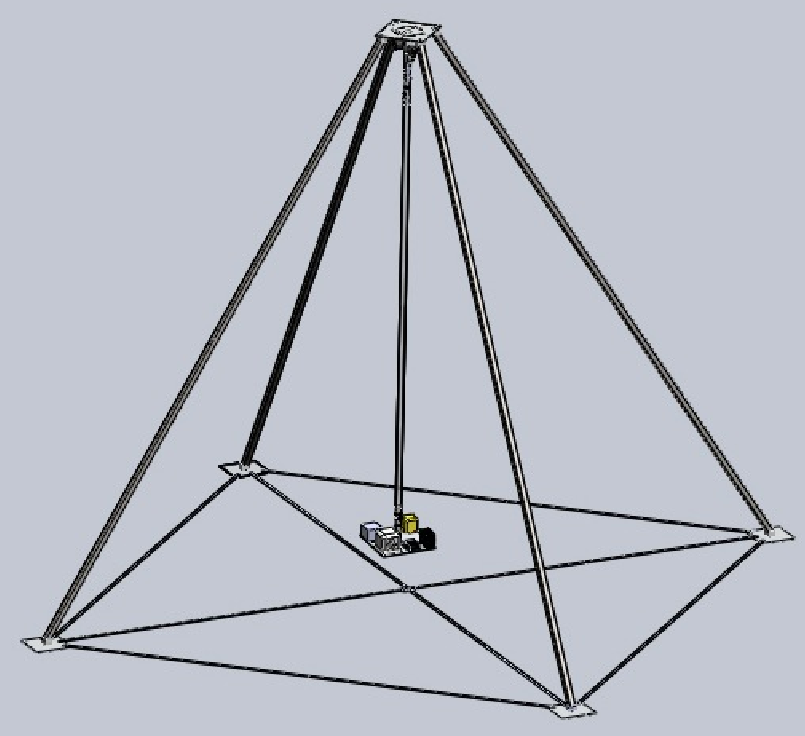
\includegraphics[height=5.5cm]{images/pendulo2.png}}
            }\hfill
            \subfloat[Diagrama de Corpo Livre]{
                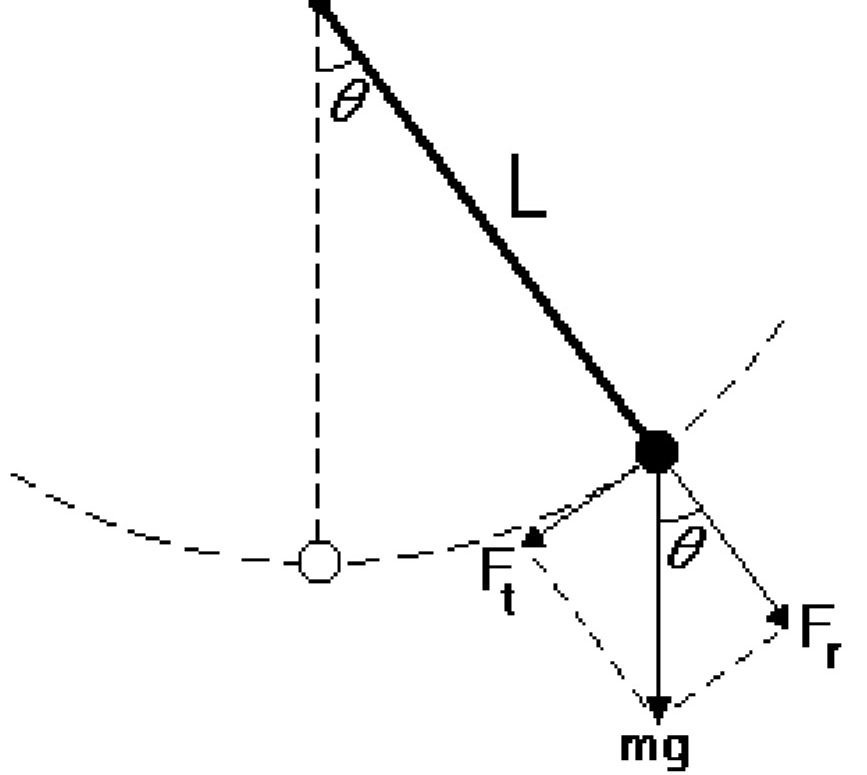
\includegraphics[height=5.5cm]{images/pendulo1.png}
            }\hfill
            \subfloat[Pêndulo Montado]{
                \frame{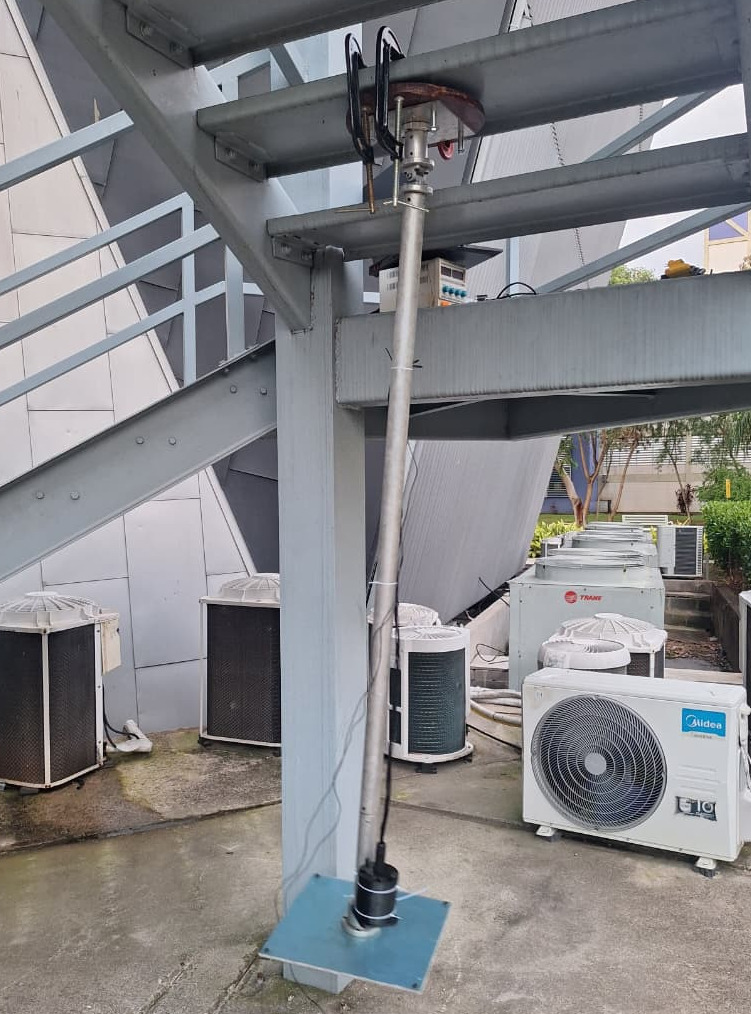
\includegraphics[height=5.5cm]{images/pendulo3.png}}
            }
            
            \label{fig:pendulo}
            \textbf{Fonte:} \href{https://nrc-publications.canada.ca/eng/view/object/?id=2b49dae2-b5b7-403b-93ba-6b03a40a230b}{House, Thomas}.
        \end{figure}
        
        O encoder foi empregado para quantificar a inclinação da haste do pêndulo em relação ao eixo vertical. O modelo adotado, E40S6-5000-6-L-5, da Smartec Automação, constitui uma versão otimizada de encoder incremental programável, caracterizado por alta resolução e robustez em ambientes adversos. Sua precisão é de 5000 pulsos por rotação, equivalente a 0,072º por pulso. Ele foi utilizado para validar a acurácia das medições realizadas pelo MRU nos testes de calibração.

        \begin{figure}[H]
            \centering
            \caption{Encoder Incremental Adotado}
            \subfloat[Dispositivo Empregado]{
                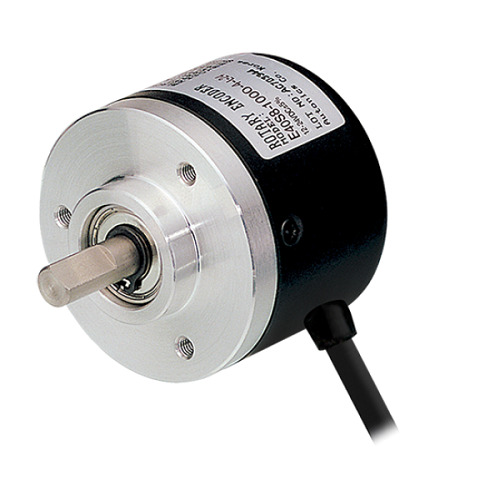
\includegraphics[height=5.5cm]{images/encoder1.png}
            }\hspace{2cm}
            \subfloat[Instalação no Pêndulo]{
                \frame{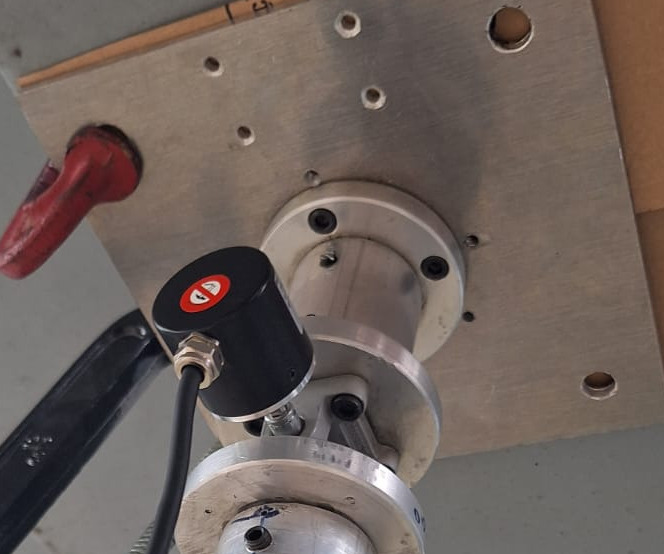
\includegraphics[height=5.5cm]{images/encoder2.png}}
            }
            
            \label{fig:graf_stew}
            \textbf{Fonte:} Autoria Própria
        \end{figure}

        Os dados angulares adquiridos serão utilizados para comparação com as variáveis medidas pelo acelerômetro e giroscópio do sensor. Essas variáveis são inferidas indiretamente a partir das leituras do encoder, com base em relações matemáticas que modelam o comportamento do pêndulo simples. Dessa forma, as variáveis inferidas são confrontadas com as obtidas diretamente, possibilitando o avanço para a etapa de calibração.

        A comparação com o pêndulo foi estendida para validar a robustez do algoritmo de alinhamento e a precisão da medição de orientação em cenários dinâmicos, assegurando a fidelidade dos dados em ambientes operacionais reais. A \autoref{fig:encoder_kernel} apresenta graficamente uma comparação simples da leitura do encoder com o giroscópio do Kernel em escala normalizada. A similaridade das curvas demonstra a robustez do método.

        \begin{figure}[H]
            \centering
            \caption{Comparação Preliminar do Sensor Kernel com Encoder}
            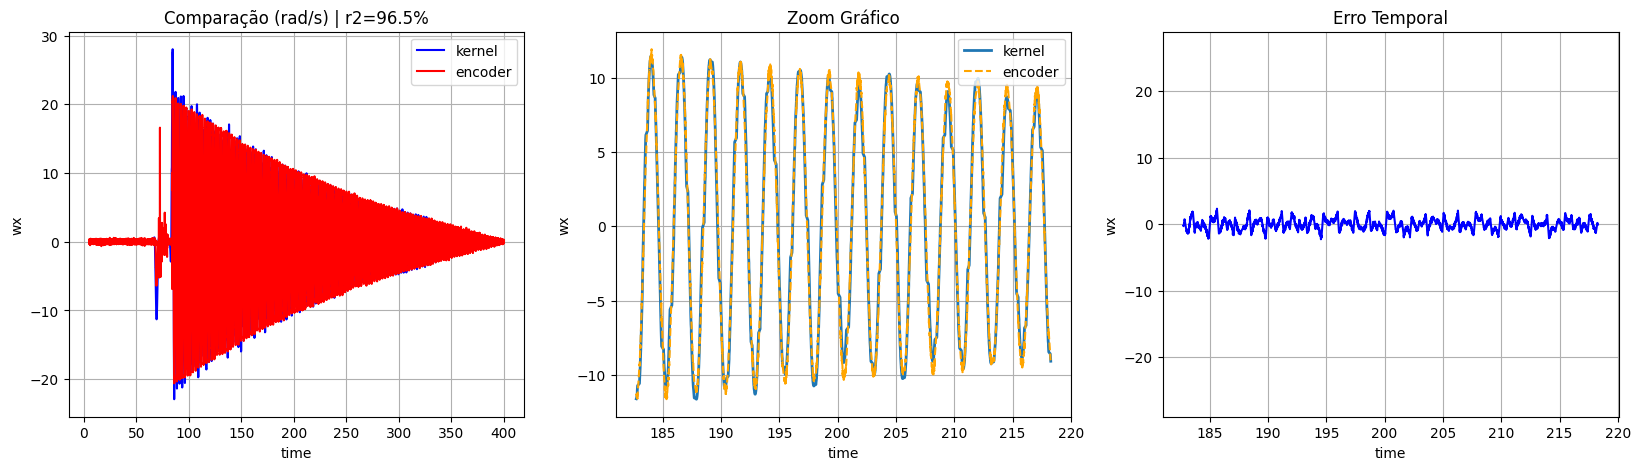
\includegraphics[width=\linewidth]{images/kernel_encoder.png}
            
            \textbf{Fonte:} Autoria Própria
            \label{fig:encoder_kernel}
        \end{figure}

        O comportamento do gráfico segue o esperado do ponto de vista físico e matemático. Ele corresponde a uma função senoidal representada pelas oscilações causadas pelo balanço do pêndulo. Além disso, há um fator de amortecimento exponencial gerado pelo atrito natural do ar. Logo, a amplitude da oscilação diminui até o pêndulo parar por completo. Esse padrão é vantajoso pois permite que os testes dinâmicos e estáticos sejam realizados de forma sequencial e natural. Dessa maneira, não são necessários motores ou impulsionadores artificiais. Portanto, há redução de custos e maior previsibilidade dos dados.

\newpage
\section{Resultados}
    A seguir, após a implementação do procedimento metodológico, os resultados obtidos por meio dos experimentos e dos estudos comparativos serão apresentados a seguir. 

    \vspace{-0.3cm}
    \subsection{Calibração}
        A calibração do dispositivo segue a metodologia já abordada anteriormente e pode ser realizada desde que as variáveis de referência sejam obtidas corretamente. Isso é viável tanto com o pêndulo simples quanto com outro dispositivo de monitoramento de alta precisão, permitindo não só a calibração, mas também a comparação e validação em relação a concorrentes do mercado, além de possibilitar instalações independentes da estrutura, pois ambos exibem o mesmo comportamento.

        A exemplo do pêndulo, a cada calibração, o dispositivo de monitoramento é alinhado com o plano de oscilação da estrutura. Ao alinhar, por exemplo, o eixo X do sensor com o plano, permite-se que o sistema obtenha medições precisas da movimentação do pêndulo e, consequentemente, ajuste seus parâmetros para leituras mais exatas. O ângulo de rotação $\phi$ medido pelo encoder é comparado com a variável $roll$, e a variação angular $\omega_x$ é comparada com a derivada do próprio ângulo $\phi$ em relação ao tempo, para se encontrar a taxa de variação angular correspondente. A Figura\autoref{fig:comp0__} mostra a instalação do pêndulo com o encoder e o MRU 5 da Kongsberg.

        \begin{figure}[H]
            \centering
            \caption{Testes Comparativos no Pêndulo com MRU 5 Kongsberg}
            \subfloat[]{
                \frame{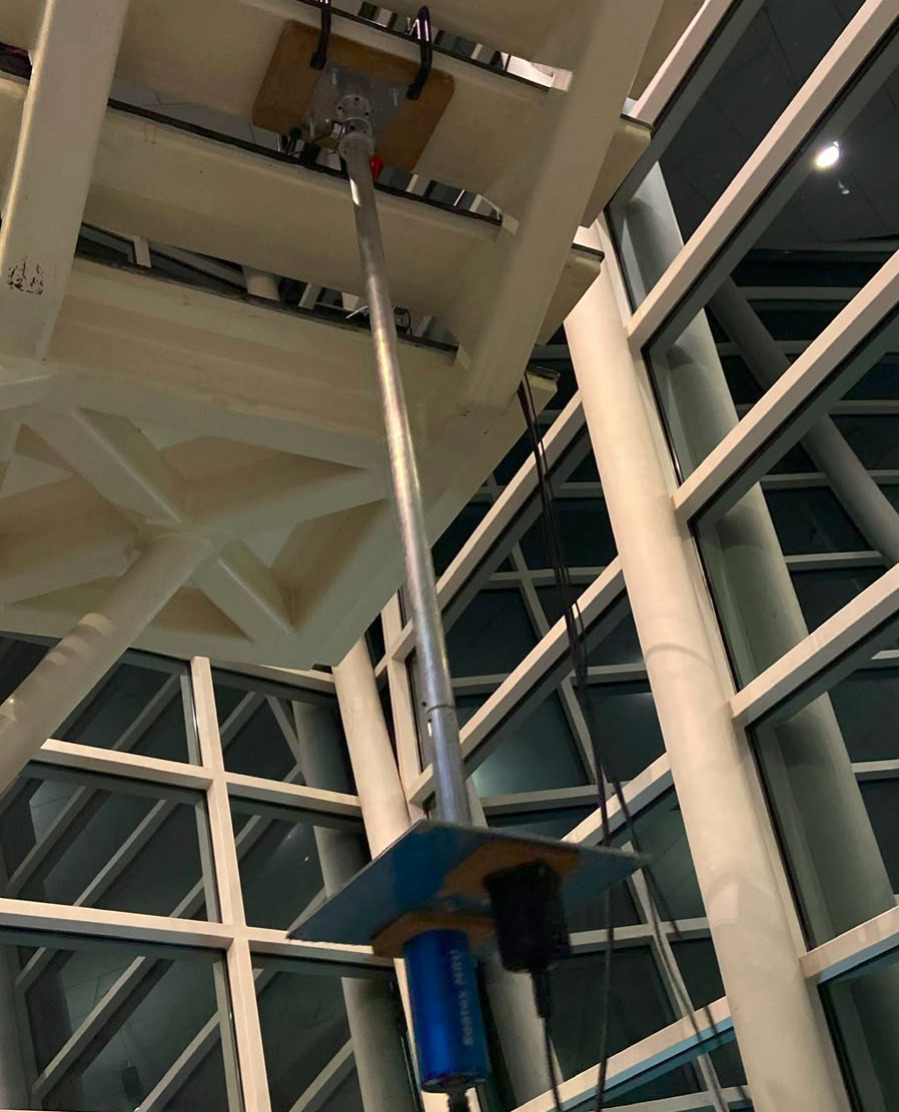
\includegraphics[height=9cm]{images/pendulo_lamce.png}}
            }\hspace{.5cm}
            \subfloat[]{
                \frame{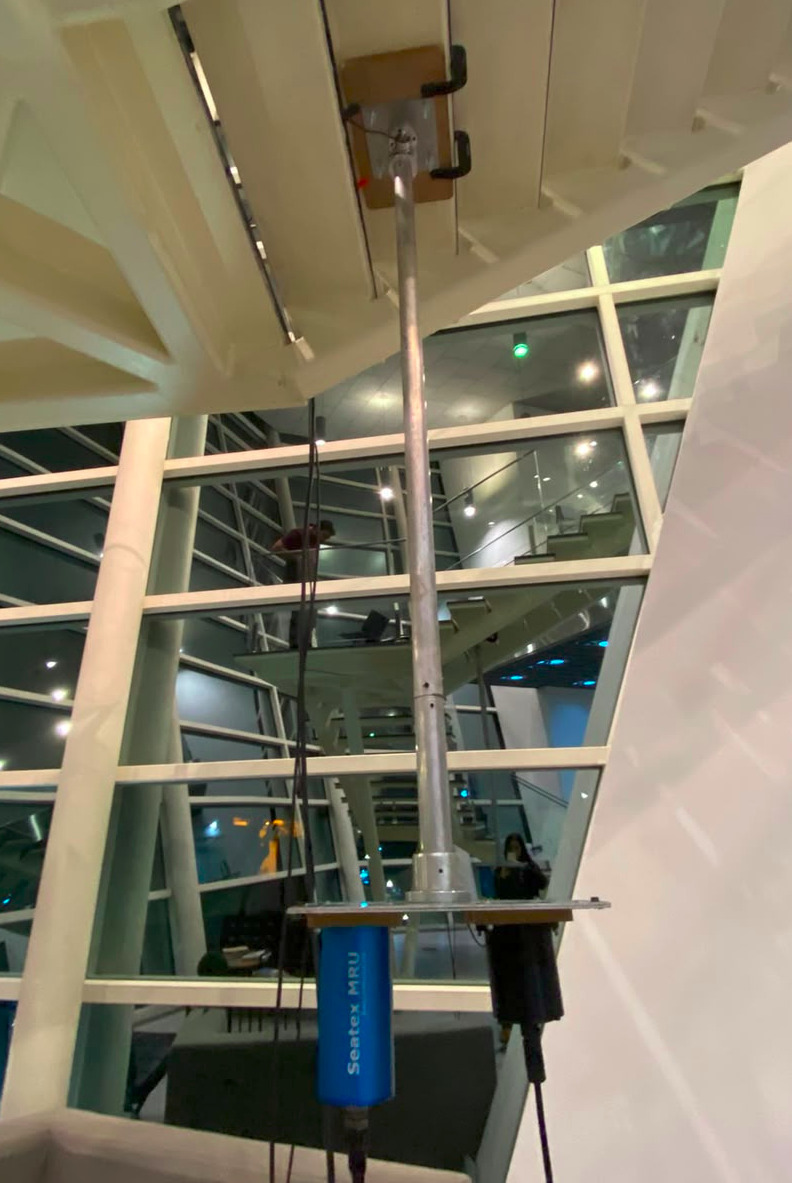
\includegraphics[height=9cm]{images/pendulo_lamce2.png}}
            }
            
            \textbf{Fonte:} Autoria Própria
            \label{fig:comp0__}
        \end{figure}

        Quando se tratando da comparação com um dispositivo concorrente no mercado, os testes dinâmicos e estáticos foram realizados com o MRU 5 da Kongsberg, referência no setor. A vantagem dessa abordagem é que os testes podem ser realizados de forma mais direta, comparando-se os dados extraídos com os do dispositivo em desenvolvimento, o que permite estabelecer uma relação linear direta entre elas e corrigir desalinhamentos em código. Esse método é de grande importância, pois será usado como principal meio para avaliar se o dispositivo em desenvolvimento é capaz de competir no mercado. A \autoref{fig:comp0_} mostra a comparação gráfica na variável de aceleração angular entre os dois dispositivos (extraídos a partir dos testes com o pêndulo), evidenciando a similaridade das curvas monitoradas.

        \begin{figure}[H]
            \centering
            \caption{Comparação do Giroscópio com o MRU 5 Kongsberg}
            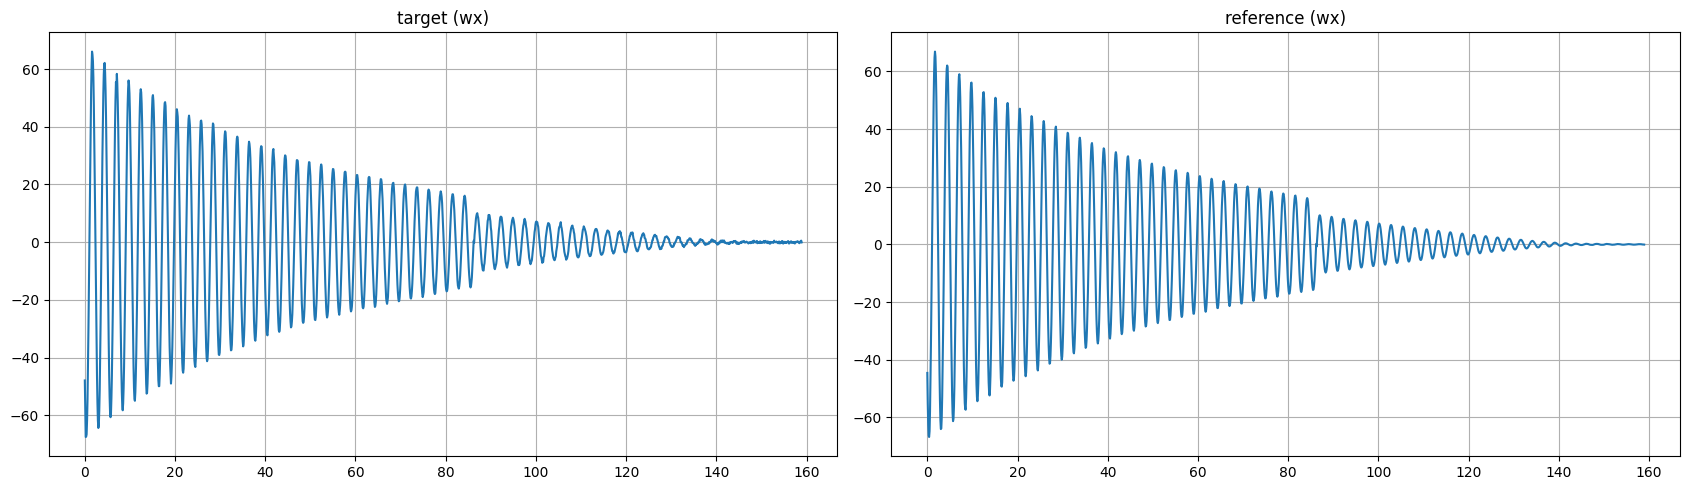
\includegraphics[width=\linewidth]{images/comp0_.png}
            
            \textbf{Fonte:} Autoria Própria
            \label{fig:comp0_}
        \end{figure}

        O processo de calibração é finalizado por meio de um ajuste linear entre a variável observada pelo sensor e a variável de referência. Após o ajuste os coeficientes de inclinação $a$ e ajuste vertical $b$ da equação da reta são armazenados na memória do próprio dispositivo e posteriormente são aplicados para corrigir as leituras, garantindo a precisão dos dados em tempo real. Ao final, a métrica de validação $R^2$ é aplicada para avaliar a acurácia entre as curvas obtidas e a de referência, garantindo a acurácia das medições. A métrica de erro é obtida de forma absoluta que é a diferença entre as duas medições e o desvio padrão amostral é usado para verificar a dispersão do erro. Outras informações estatísticas são calculadas, como erro mínimo e máximo, média e mediana. A \autoref{fig:calib01} mostra as métricas numéricas junto à análise gráfica, onde se pode observar uma alta similaridade numérica entre os dois dispositivos, o que pode ser validado pela aproximação de 99.9\% pelo $R^2$ Score.

        \begin{figure}[H]
            \centering
            \caption{Calibração Preliminar Gerada a partir de Testes no Pêndulo}
            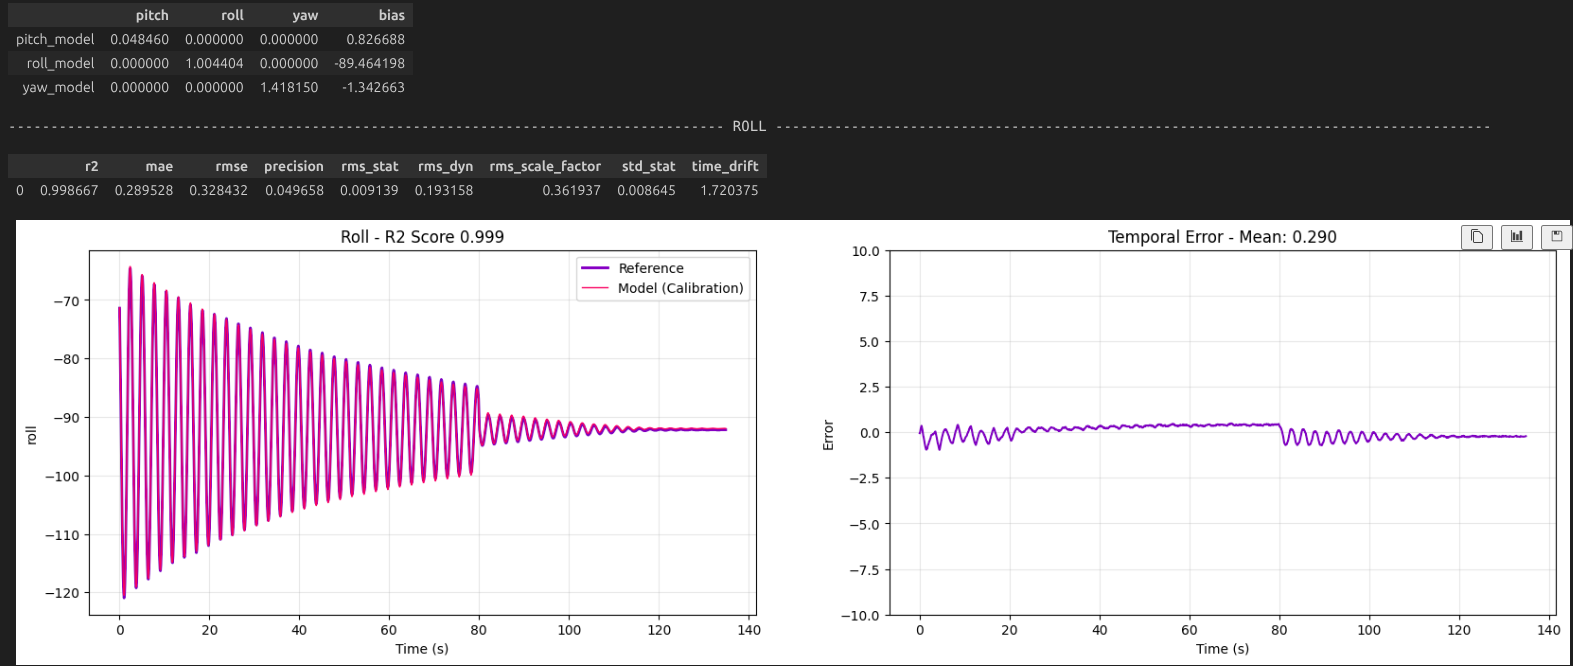
\includegraphics[width=\linewidth]{images/calib01.png}
            
            \textbf{Fonte:} Autoria Própria
            \label{fig:calib01}
        \end{figure}

        As informações estatísticas que comparam os dados do sensor aos de referência são, portanto, armazenadas, e um relatório de calibração é gerado em formato PDF. Esse relatório, mostrado na Figura\autoref{fig:certificado}, apresenta as métricas alcançadas, comparando-as diretamente aos critérios de aceitação, definidos como os limiares mínimos das variáveis para qualificação do sensor no mercado, os quais foram ajustados conforme referências de mercado a serem discutidas na seção subsequente.
        
        \begin{figure}[H]
            \centering
            \caption{Certificado de Calibração}

            \subfloat[Modelo Kongsberg]{
                \frame{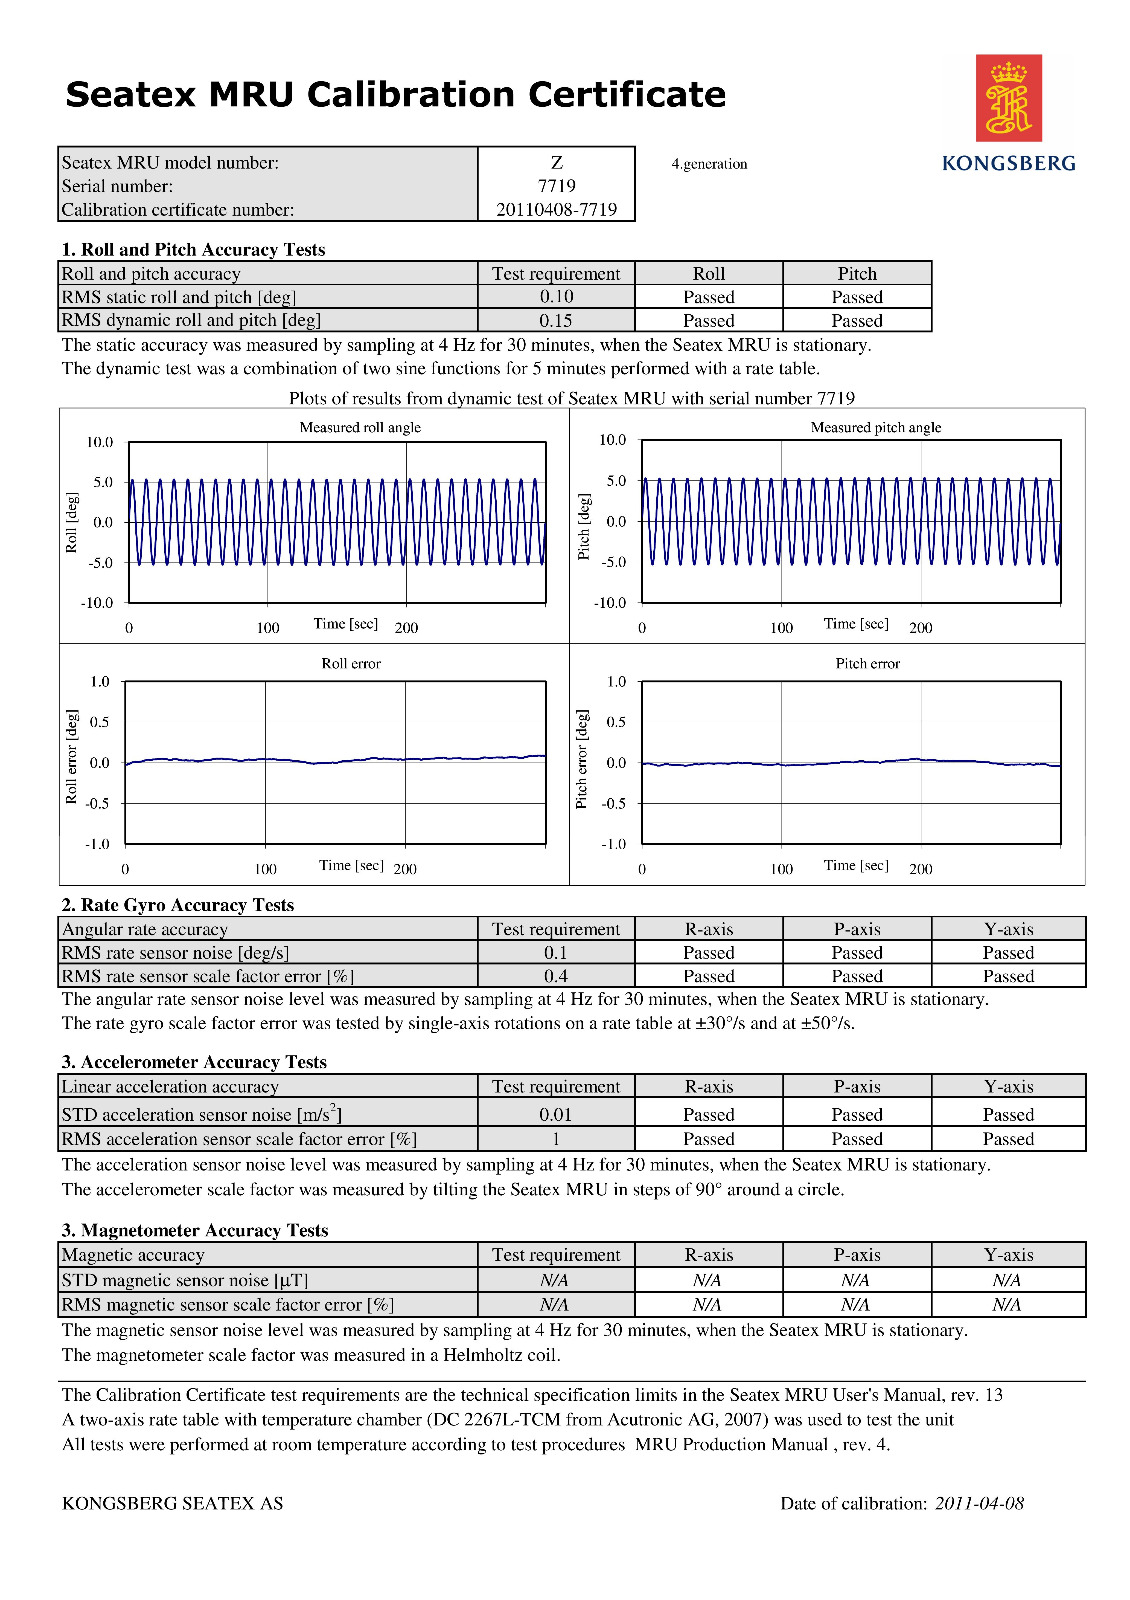
\includegraphics[height=11.4cm]{images/kongsberg_certificado.png}}
            }\hfill
            \subfloat[Modelo Measure]{
                \frame{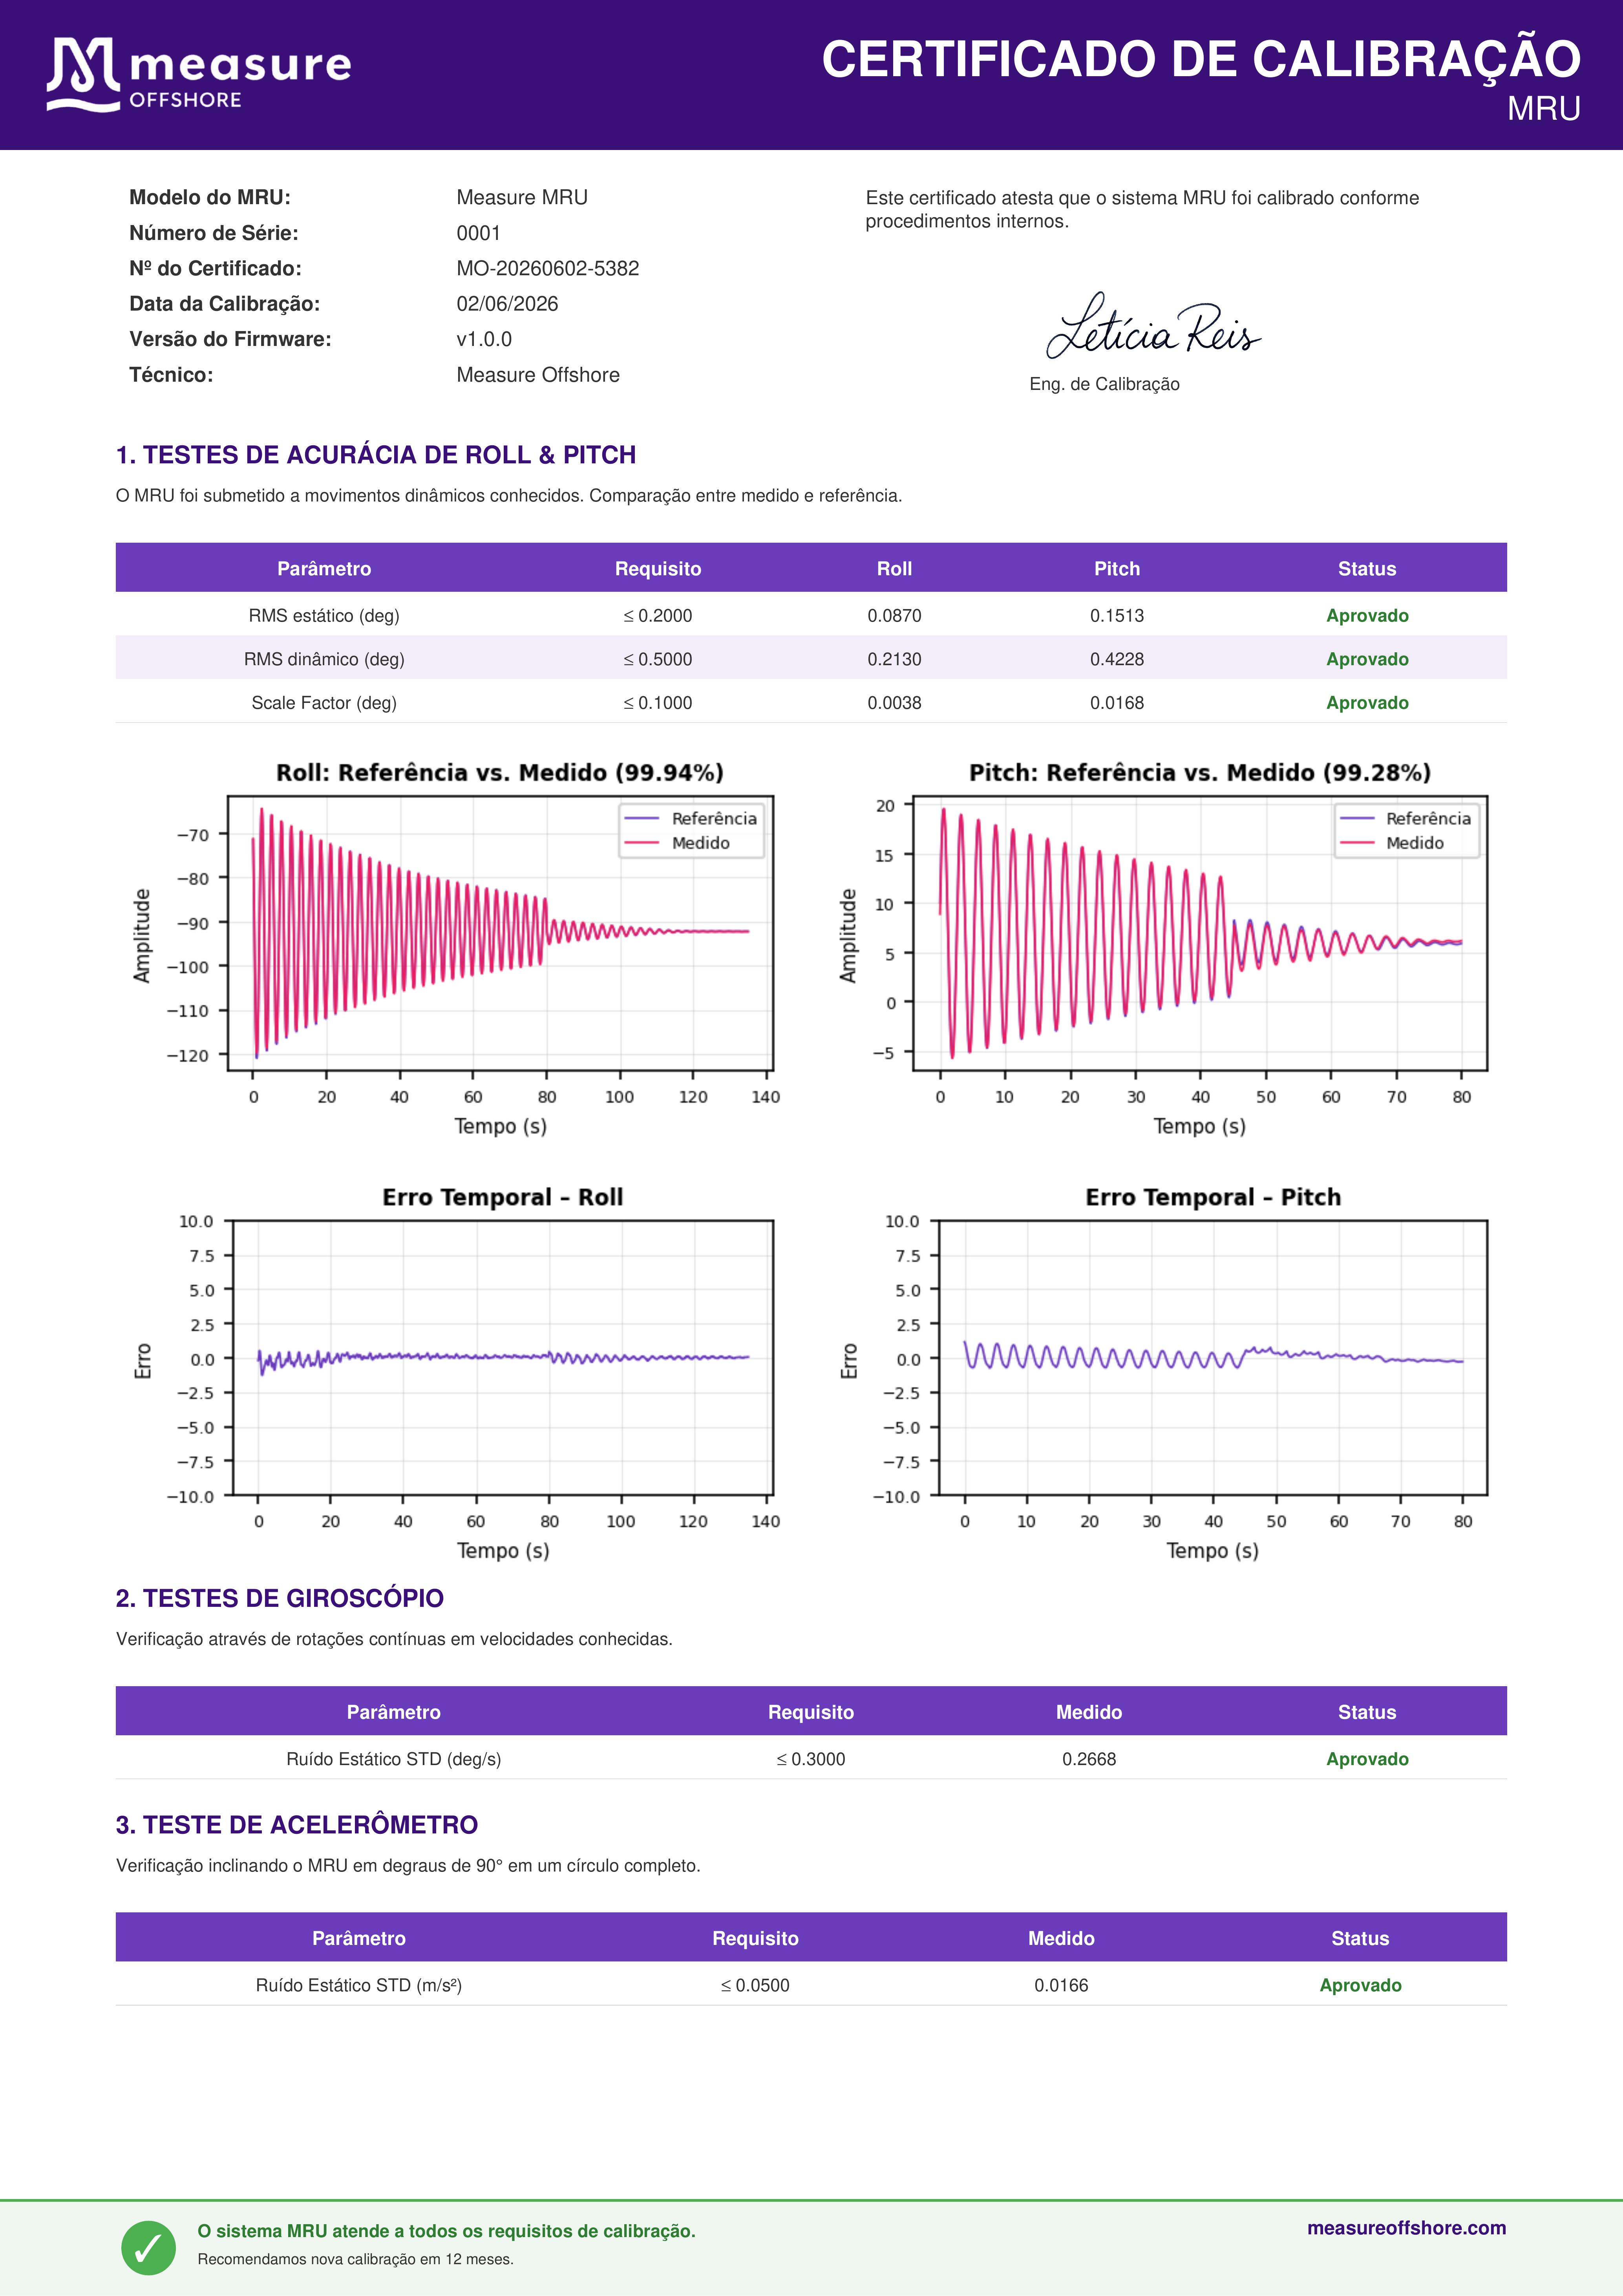
\includegraphics[height=11.4cm]{images/img_1.jpg}}
            }
            
            \textbf{Fonte:} Autoria Própria
            \label{fig:certificado}
        \end{figure}

        A avaliação comparativa entre os certificados evidencia similaridades no desempenho dos equipamentos. Contudo, o modelo Kongsberg apresenta uma precisão muito superior. Essa diferença reflete de forma direta o alto investimento financeiro e a qualidade dos sensores adotados no aparelho. O equipamento comercial atua exclusivamente como uma base de referência para avaliar a eficiência do sensor de baixo custo criado neste projeto. Além disso, a análise técnica busca confirmar a viabilidade do novo dispositivo no ambiente offshore. Portanto, o objetivo central é garantir o cumprimento das exigências impostas pelas normas regulatórias do setor, mesmo diante da precisão reduzida do modelo desenvolvido.


    \subsection{Validação de Mercado}
        Antes de comentar sobre os dados extraídos uma comparação preliminar foi feita ao se analisar os datasheets do sensor Kernel utilizado com relação aos dois maiores concorrentes de mercado sendo estes o MRU 4 e MRU 5 da empresa Kongsberg, sendo o 5 alugado para comparação direta. A \autoref{tab:sensores} apresenta a comparação direta entre o sensor Kernel e os modelos de referência da Kongsberg.

        \begin{center}
        \centering\footnotesize
        {\renewcommand{\arraystretch}{1.2}
        \begin{longtable}{|c|c|c|c|c|}
            \caption{Comparativo de Especificações dos Sensores Inerciais} \label{tab:sensores}\\
            \hline
                \fcol{.25}{\textbf{Parâmetro}} & 
                \col{.3}{\textbf{Descrição}} & 
                \col{.15}{\textbf{KERNEL-120}} & 
                \col{.15}{\textbf{Kongsberg MRU 4}} & 
                \col{.15}{\textbf{Kongsberg MRU 5}} \\
            \hline 
                \fcol{.25}{Pitch \& Roll Static (deg)} & 
                \col{.3}{Precisão de inclinação (estática) quando parado} & 
                \col{.15}{0.05} & 
                \col{.15}{0.05} & 
                \col{.15}{0.02} \\
            \hline
                \fcol{.25}{Pitch \& Roll Dynamic (deg)} & 
                \col{.3}{Precisão de inclinação (dinâmica) em movimento} & 
                \col{.15}{0.05} & 
                \col{.15}{0.05} & 
                \col{.15}{0.02} \\
            \hline
                \fcol{.25}{Heave Accuracy (cm/\%)} & 
                \col{.3}{Precisão da medição do movimento vertical (arfar)} & 
                \col{.15}{N/A} & 
                \col{.15}{5 cm ou 5\%} & 
                \col{.15}{5 cm ou 5\%} \\
            \hline
                \fcol{.25}{Gyro Bias Instability (deg/hr)} & 
                \col{.3}{Estabilidade do desvio do giroscópio no tempo} & 
                \col{.15}{2.0} & 
                \col{.15}{1.0} & 
                \col{.15}{0.15} \\
            \hline
                \fcol{.25}{Gyro ARW (deg/$\sqrt{\mathrm{hr}}$)} & 
                \col{.3}{Ruído aleatório que afeta a precisão do ângulo} & 
                \col{.15}{0.3} & 
                \col{.15}{0.05} & 
                \col{.15}{0.01} \\
            \hline
                \fcol{.25}{Accel Bias Instability (mg)} & 
                \col{.3}{Estabilidade do desvio do acelerômetro (bias)} & 
                \col{.15}{0.05} & 
                \col{.15}{0.2} & 
                \col{.15}{0.1} \\
            \hline
                \fcol{.25}{Accel VRW (m/s/$\sqrt{\mathrm{hr}}$)} & 
                \col{.3}{Ruído aleatório que afeta a precisão da velocidade} & 
                \col{.15}{0.06} & 
                \col{.15}{0.01} & 
                \col{.15}{0.012} \\
            \hline
                \fcol{.25}{Accel Range (g)} & 
                \col{.3}{Faixa máxima de aceleração sem saturação} & 
                \col{.15}{$\pm$40 / $\pm$90} & 
                \col{.15}{$\pm$5.1} & 
                \col{.15}{$\pm$3.06} \\
            \hline
                \fcol{.25}{Heading Accuracy (deg)} & 
                \col{.3}{Precisão da medição de rumo ou direção (proa)} & 
                \col{.15}{N/A} & 
                \col{.15}{0.3} & 
                \col{.15}{N/A} \\
            \hline
                \fcol{.25}{Power Consumption (W)} & 
                \col{.3}{Consumo de potência elétrica em operação} & 
                \col{.15}{0.6} & 
                \col{.15}{6.0} & 
                \col{.15}{9.0} \\
            \hline
                \fcol{.25}{Interface} & 
                \col{.3}{Meio físico e protocolo de comunicação} & 
                \col{.15}{RS-422} & 
                \col{.15}{Serial / Ethernet} & 
                \col{.15}{Serial / Ethernet} \\
            \hline
                \fcol{.25}{Weight (kg)} & 
                \col{.3}{Massa total do dispositivo} & 
                \col{.15}{0.01} & 
                \col{.15}{2.5} & 
                \col{.15}{2.2} \\
            \hline
                \fcol{.25}{Dimensions (mm)} & 
                \col{.3}{Tamanho físico (D $\times$ H ou L $\times$ W $\times$ H)} & 
                \col{.15}{28.4 $\times$ 19.5 $\times$ 10.5} & 
                \col{.15}{105 $\times$ 204} & 
                \col{.15}{105 $\times$ 140} \\
            \hline
                \fcol{.25}{Op. Temp Range (°C)} & 
                \col{.3}{Faixa de temperatura de operação garantida} & 
                \col{.15}{-40 to +85} & 
                \col{.15}{-5 to +55} & 
                \col{.15}{-5 to +55} \\
            \hline
        \end{longtable}
        }
        
        \normalsize
        \textbf{Fonte:} \cite{inertiallabs_kernel120, kongsberg_mru5_install_2006, kongsberg_recal_2024, kongsberg_mru4_legacy, kongsberg_mru5_datasheet}
    \end{center}
        
        Os dados confirmam maior aproximação do sensor Kernel ao MRU 4 da Kongsberg, ambos com valores de pitch e roll de 0,05° RMS, posicionando o protótipo no mesmo patamar do modelo anterior, enquanto o MRU 5 exibe precisão superior de 0,002° RMS, destinado a aplicações mais exigentes, o que resulta em um maior custo. Apesar de o KERNEL apresentar métricas inferiores ao MRU 5, uma vantagem estratégica reside no uso do MRU 5 como gabarito por referência em testes estáticos e dinâmicos. Essa calibração permite comparações rigorosas e afirmações confiáveis sobre o desempenho do sensor, validando sua competitividade no mercado.
        
        Não obstante, para uma validação empírica eficaz, conduziram-se testes comparativos em campo, sob condições dinâmicas reais. Tal abordagem permite uma comparação equânime, tanto gráfica quanto numérica, confirmando se o projeto satisfaz efetivamente os requisitos. A principal métrica de comparação entre as duas curvas é o $R^2$ Score, que mede a proporção da variância total dos dados explicada pelo modelo; é calculado subtraindo da unidade a razão entre a soma dos quadrados dos resíduos (variância não explicada) e a soma total dos quadrados (variância total). Valores próximos de 1 indicam alto grau de ajuste entre as curvas. As figuras a seguir apresentam comparações diretas entre os dois dispositivos.
        
        \begin{figure}[H]
            \centering
            \caption{Comparação Geral - Testes do Pêndulo Measure/Kongsberg}
            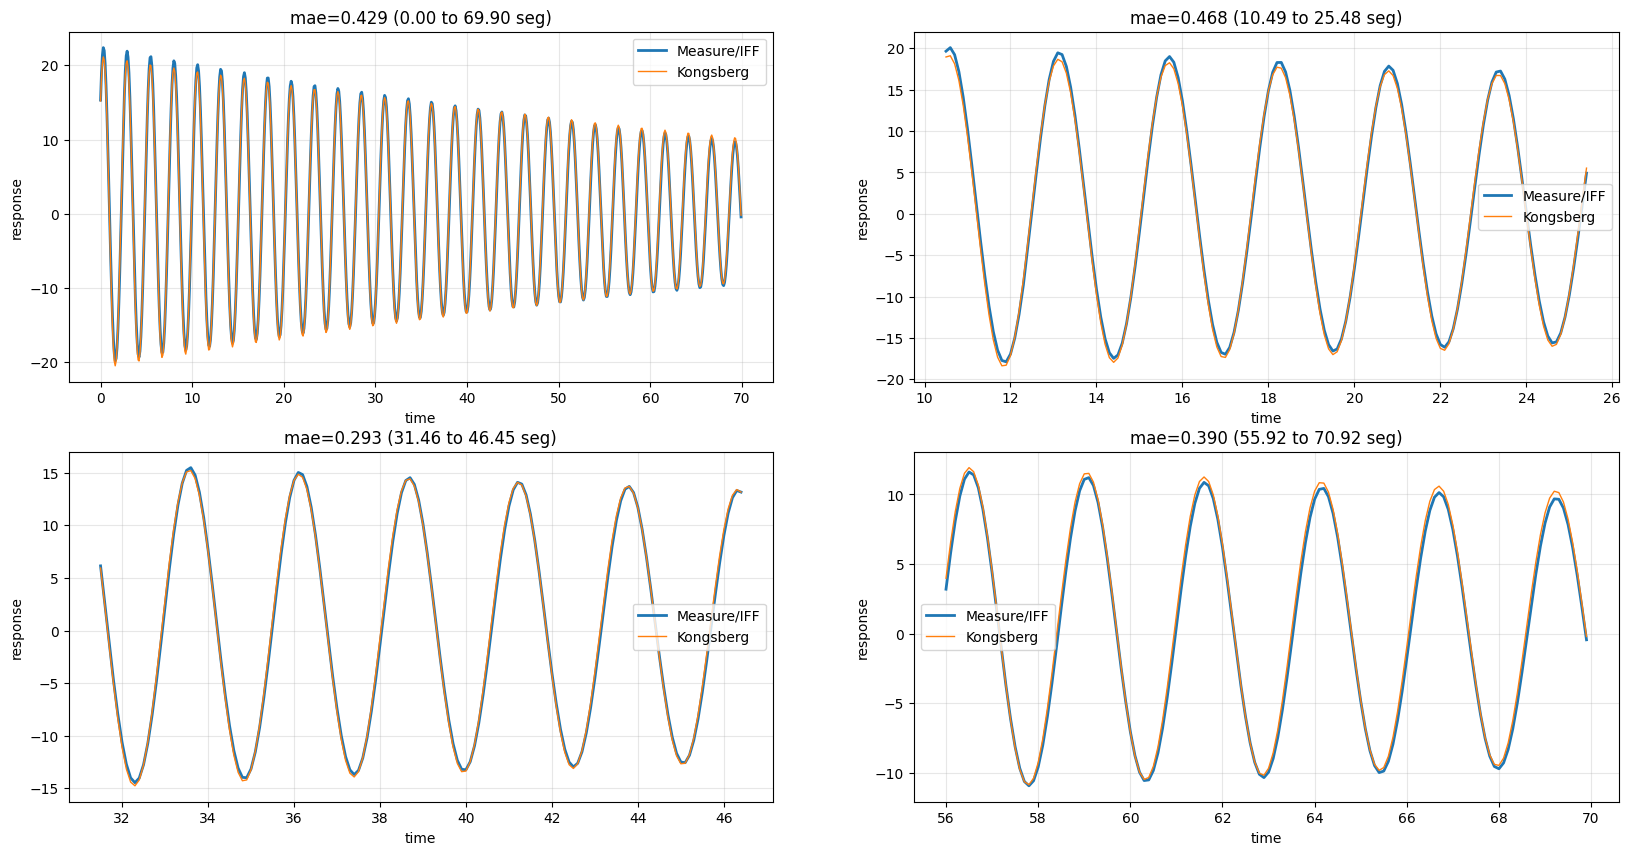
\includegraphics[width=\linewidth]{images/comp0.png}
            
            \textbf{Fonte:} Autoria Própria
            \label{fig:comp01}
        \end{figure}
        
        A avaliação da precisão estática e dinâmica desses dados seguiu um método semelhante ao da calibração com o pêndulo; para isso, aplicou-se uma interpolação linear simples, que "preenche"\ os espaços entre os pontos de dados com linhas retas, combinada com um ajuste de curva, permitindo comparar os resultados em faixas de amplitude iguais. Além disso, testou-se se é possível obter desempenhos similares ao calibrar o dispositivo com um MRU mais avançado. Os gráficos subsequentes mostram o erro absoluto para cada valor registrado entre os dispositivos, o que permite observar a alta similaridade entre as funções.

        \begin{figure}[H]
            \centering
            \caption{Comparação de Medidas - Roll}
            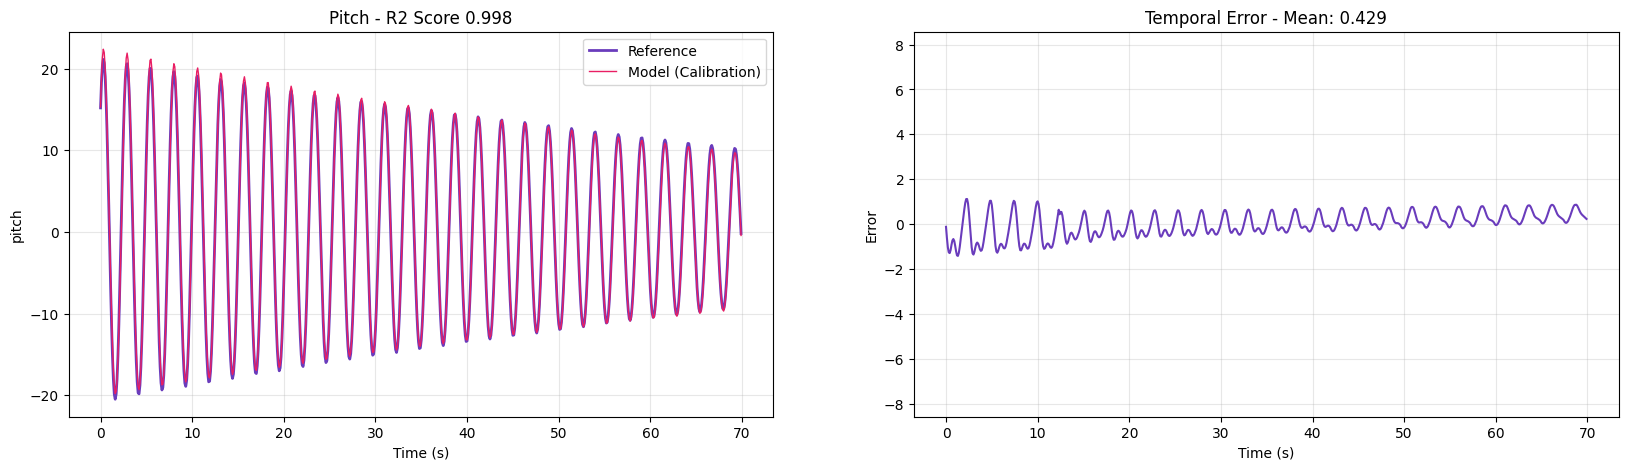
\includegraphics[width=\linewidth]{images/comparacao02.png}
            
            \textbf{Fonte:} Autoria Própria
            \label{fig:comp01}
        \end{figure}

        \begin{figure}[H]
            \centering
            \caption{Comparação de Medidas - Pitch}
            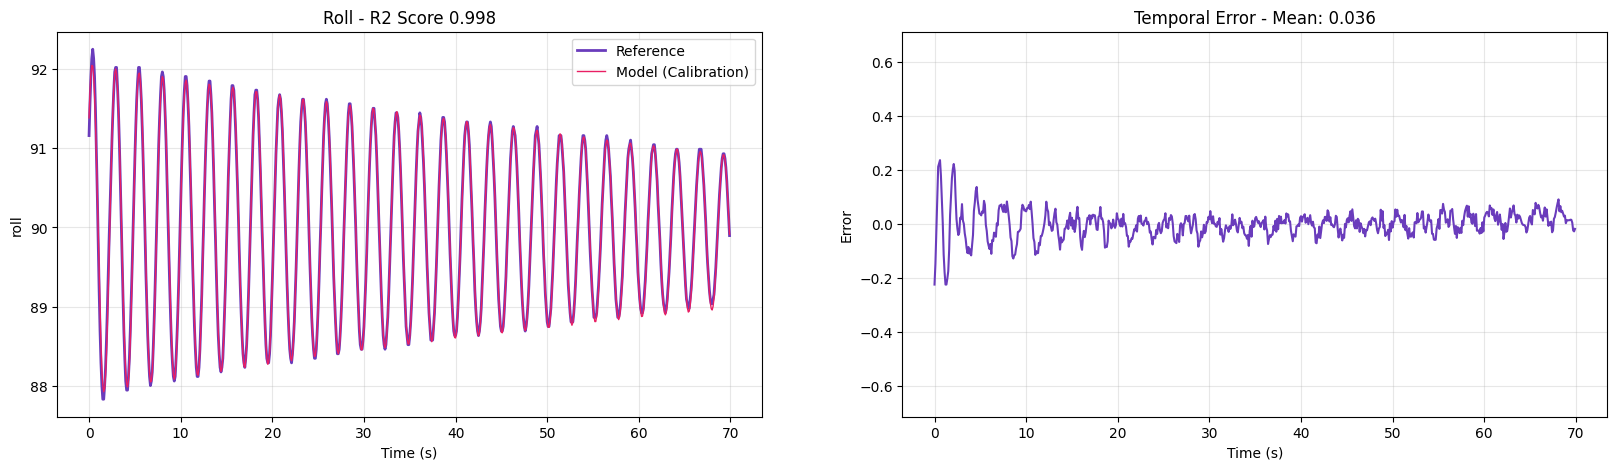
\includegraphics[width=\linewidth]{images/comparacao1.png}
            
            \textbf{Fonte:} Autoria Própria
            \label{fig:comp02}
        \end{figure}
        
        Com as principais comparações realizadas graficamente, procedeu-se ao cálculo de variáveis estatísticas para quantificar de forma precisa a similaridade entre os dispositivos KERNEL e o MRU Kongsberg. Além do $R^2$, que já explicado, também foram adotados o MAE, calculado como a média dos valores absolutos das diferenças entre os valores previstos e observados, proporcionando uma medida intuitiva da magnitude média dos erros sem considerar o sinal; o RMSE, obtido pela raiz quadrada da média dos quadrados dos erros residuais, o qual penaliza mais fortemente os erros maiores devido à elevação ao quadrado. A tabela a seguir apresenta a comparação quantitativa entre o protótipo desenvolvido e o padrão de mercado, com base nos dados coletados experimentalmente no mesmo teste realizado no gráfico acima.
        
        \begin{center}
            \centering\footnotesize
            {\renewcommand{\arraystretch}{1.2}
            \begin{longtable}{|c|c|}
                \caption{Resultados das Métricas Estatísticas} \label{tab:metricas}\\
                \hline
                    \fcol{.50}{\textbf{Métrica Estatística}} & 
                    \col{.50}{\textbf{Valor Obtido}} \\
                \hline 
                    \fcol{.50}{$R^2$} & 
                    \col{.50}{} \\
                \hline
                    \fcol{.50}{\textbf{MAE}} & 
                    \col{.50}{} \\
                \hline
                    \fcol{.50}{\textbf{RMSE}} & 
                    \col{.50}{} \\
                \hline
                    \fcol{.50}{\textbf{Max Error}} & 
                    \col{.50}{} \\
                \hline
            \end{longtable}
            }
        
            \normalsize
            \textbf{Fonte:} Autor
        \end{center}
        
       Apesar das diferenças construtivas, o sensor Kernel exibiu valores de MAE e RMSE altamente competitivos, validando assim sua aplicação em ambientes offshore conforme os critérios de aceitação.

\section{Próximos Passos}
    O escopo inicial do projeto foi concluído ao estabelecer uma metodologia de calibração baseada no pêndulo simples. Contudo, essa abordagem ainda enfrenta algumas dificuldades notáveis, como o atrito com o ar e as complicações de instalação devido ao tamanho e peso da estrutura. Logo, para maximizar a precisão, a repetibilidade e o controle da plataforma, novas soluções foram elaboradas. Esses métodos alternativos ainda se encontram em estágio inicial, no entanto se mostraram promissores, uma vez que o foco principal dessas mudanças é aprimorar a calibração e garantir uma precisão superior ao modelo anterior.

    Dessa forma, uma nova plataforma de calibração foi desenvolvida, que consiste em uma mesa motorizada com rotação em dois eixos para garantir uma aferição mais precisa. A movimentação ocorre por meio de comandos diretos aos motores de passo instalados na estrutura física. Além disso, o equipamento permite a execução de qualquer movimento previamente programado pelo usuário. A angulação pode ser medida de forma direta por um encoder. Como alternativa, ela também pode ser inferida a partir dos passos executados pelos motores a cada instrução recebida. Logo, a máquina viabiliza o monitoramento contínuo do pitch e do roll, que representam as angulações relativas de cada eixo. O modelo físico atual já está completamente construído e funcional. Adicionalmente, os primeiros testes de validação com o equipamento já foram realizados.

    \begin{figure}[H]
        \centering
        \caption{Testes Protótipo com Mesa Motorizada}
        \subfloat[]{
            \frame{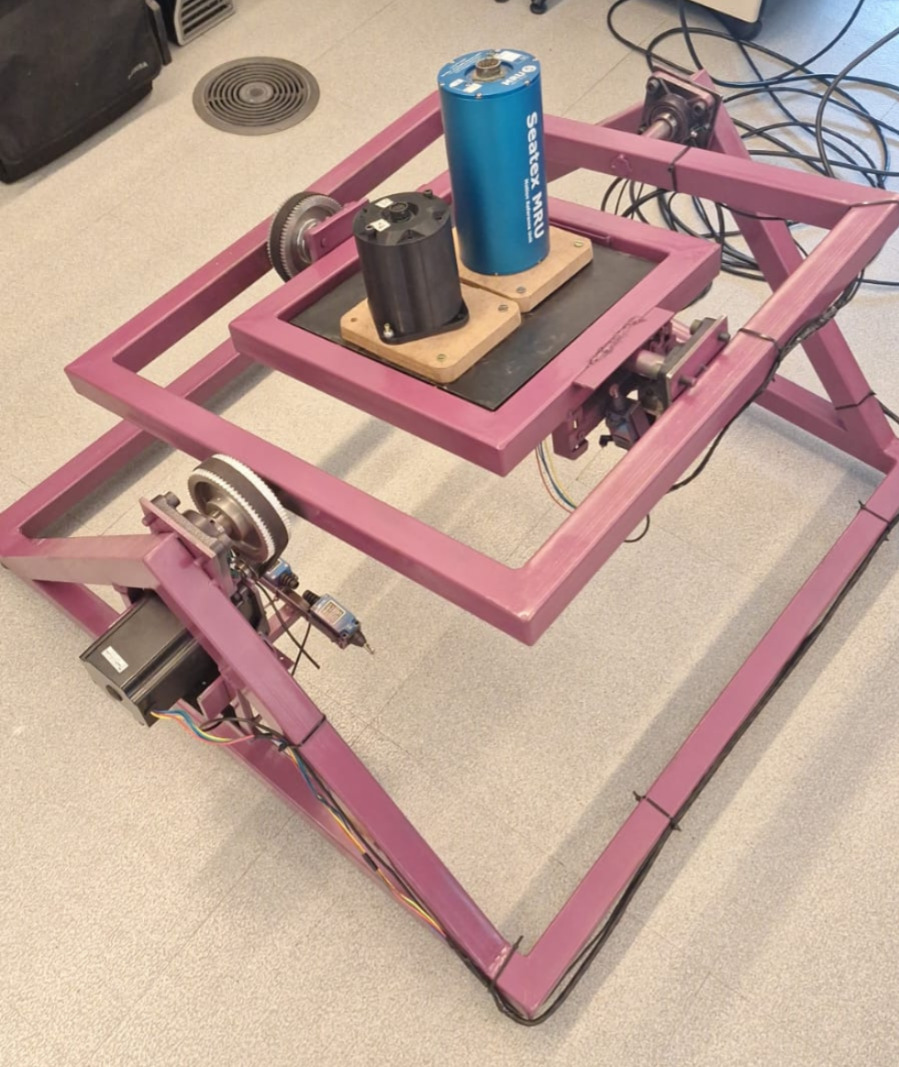
\includegraphics[height=7cm]{images/mesa1.png}}
        }\hspace{.5cm}
        \subfloat[]{
            \frame{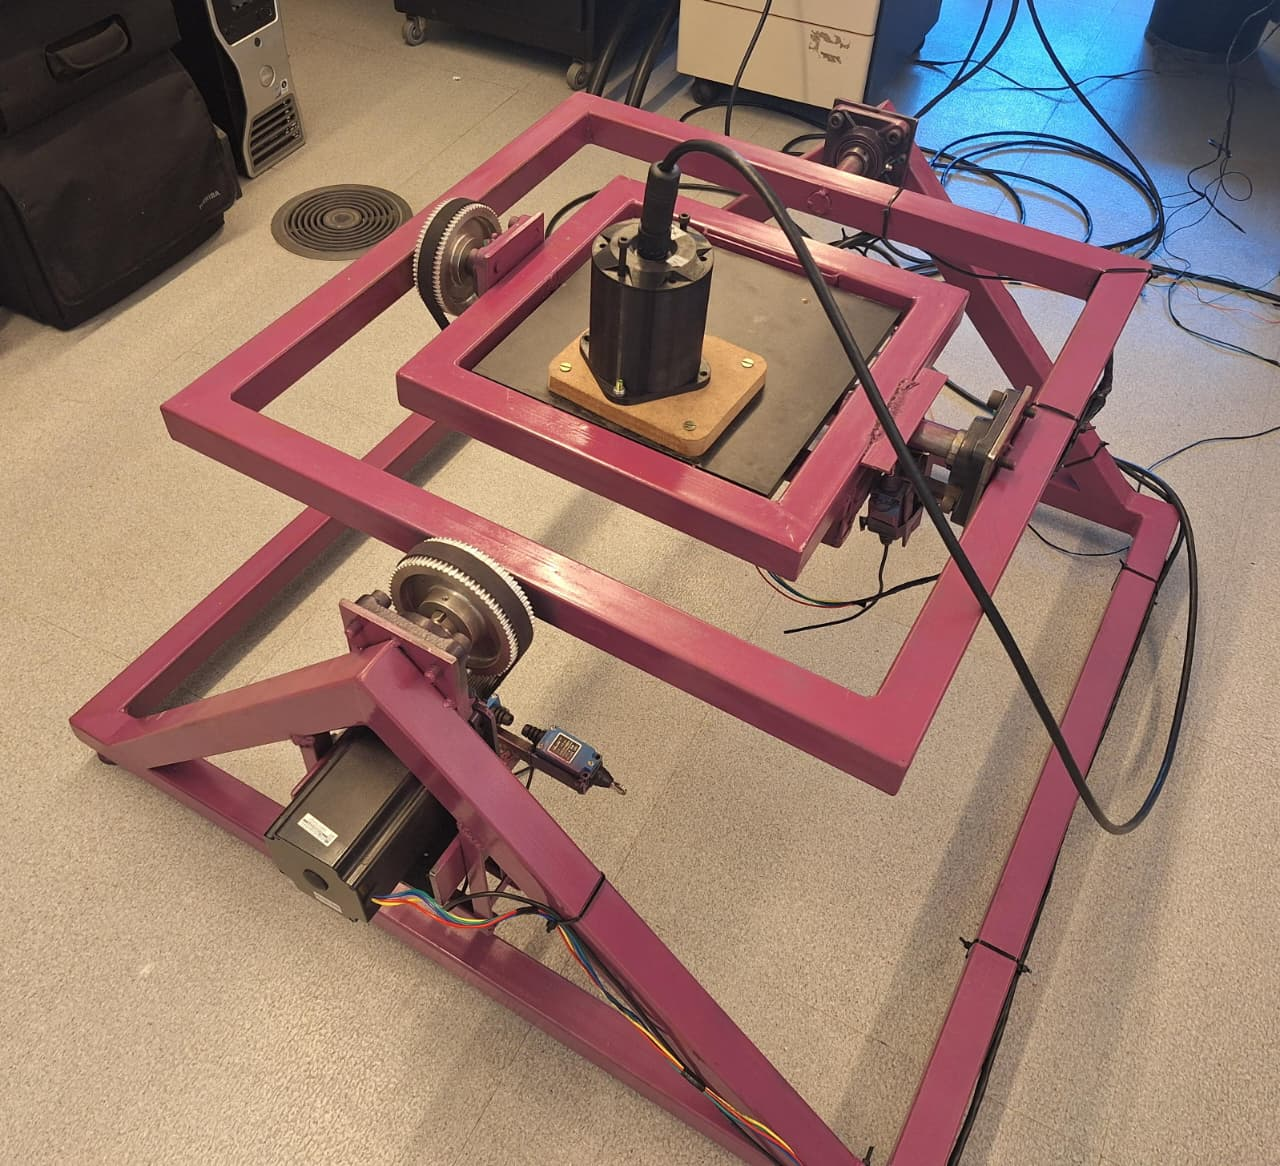
\includegraphics[height=7cm]{images/mesa2.png}}
        }
        
        \textbf{Fonte:} Autoria Própria
        \label{fig:comp0__}
    \end{figure}

    Os resultados preliminares numéricos e gráficos se mostram bastante promissores em relação à similaridade entre os dados de referência e os valores reais coletados durante as medições. O comportamento do ângulo estimado apresenta uma correspondência adequada com o valor monitorado, sendo esta dinâmica representada por simples senoides nos dois eixos com os motores acoplados. Além disso, a nova configuração estrutural oferece vantagens operacionais significativas durante a execução dos testes estáticos. Agora, com a mesa firmemente sustentada no chão, ruídos ambientais como correntes de vento ou pequenas trepidações não são mais capazes de gerar grandes divergências nos resultados. Consequentemente, o sistema atual minimiza os distúrbios de leitura e corrige uma limitação importante, visto que o método de aferição por pêndulo era extremamente suscetível a essas interferências externas.
    
    \begin{figure}[H]
        \centering
        \caption{Comparação de Medidas - Mesa Motorizada}
        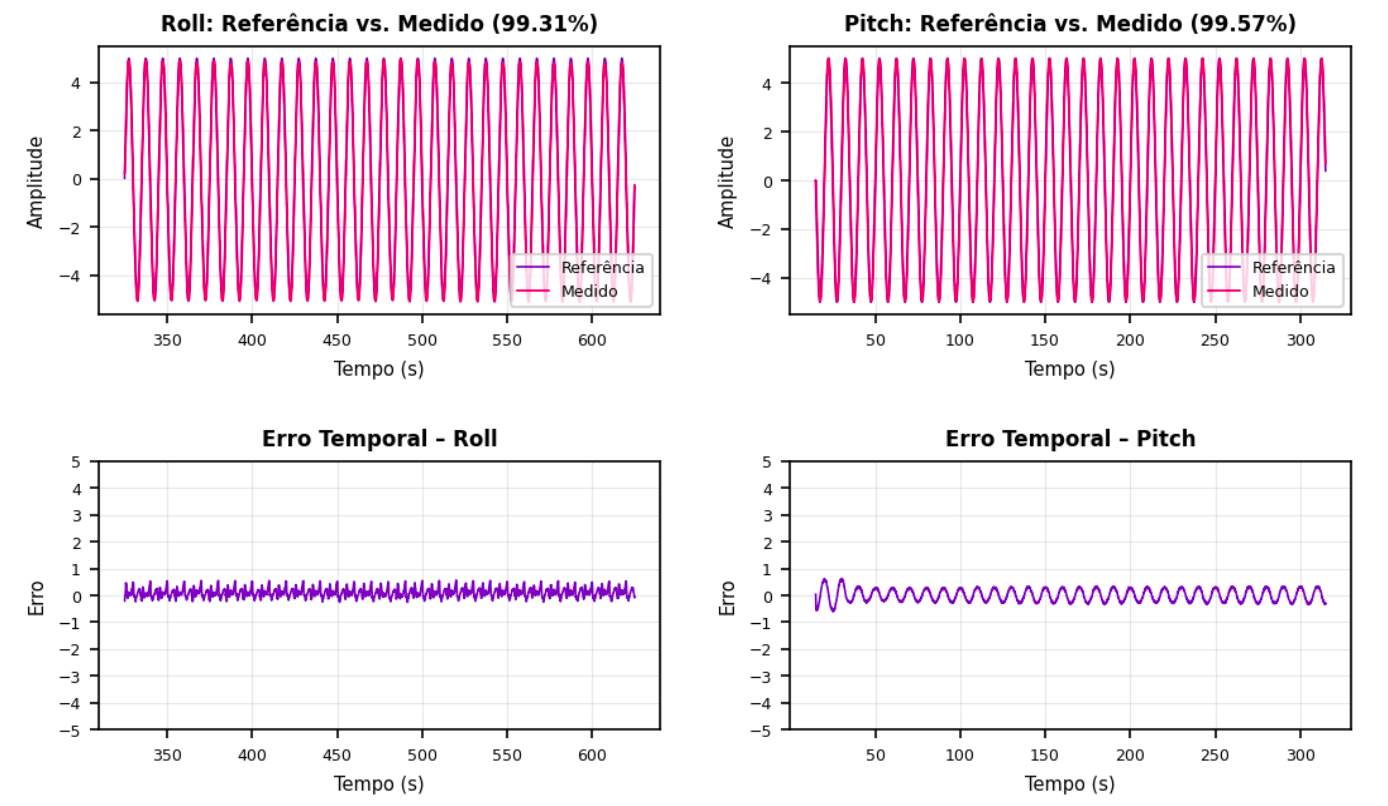
\includegraphics[width=\linewidth]{images/mesa_graphs.png}
        
        \textbf{Fonte:} Autoria Própria
        \label{fig:comp02}
    \end{figure}

    A expectativa no longo prazo é que todas essas metodologias e conceitos sejam plenamente consolidados para garantir uma base estrutural mais forte. Dessa forma, o objetivo principal das novas implementações é transformar o sistema de monitoramento em uma solução ideal, garantindo assim uma posição altamente competitiva no mercado atual. Além disso, essa evolução contínua visa assegurar que a tecnologia seja amplamente comercializada e atenda com eficácia às rigorosas demandas do setor. Portanto, os resultados globais demonstram um avanço estratégico e importante do projeto rumo aos elevados níveis de precisão, confiabilidade e robustez operacional.


\section{Conclusão}
    Diante do exposto, torna-se evidente que o dispositivo desenvolvido atende aos requisitos de desempenho para monitoramento de movimentos em helidecks e guindastes offshore, posicionando-se como uma alternativa viável e competitiva aos sistemas comerciais existentes. A sua robustez e precisão, mesmo com tecnologias de menor custo, demonstram a potencialidade para implementação em larga escala. 
    
    O procedimento de calibração do sensor Kernel permitiu verificar a fidelidade dos dados obtidos em comparação com o sistema de referência MRU Kongsberg, confirmando a acurácia das medições de pitch, roll e heave sob condições controladas e simuladas. O pêndulo foi a estrutura principal de testes de campo e que através do encoder rotativo foi possível correlacionar as medidas de rotação, validando assim a capacidade do KERNEL de registrar movimentos angulares com elevada precisão. 
    
    Foram realizados testes estáticos e dinâmicos de forma exaustiva. Implementações futuras, como algoritmos de aprendizado de máquina e novos filtros, poderão ser incorporadas posteriormente para elevar ainda mais a confiabilidade. Isso será possível utilizando os dados obtidos por meio do software HMS elaborado pela equipe, que possibilita a coleta via cabos RS422 com conversor para USB. Essa abordagem garante a integridade da comunicação de dados e minimiza a latência, essenciais para aplicações de monitoramento em tempo real.
    
    A estrutura final em 3D foi fabricada e integrada ao dispositivo, incorporando uma placa de circuito impresso dedicada que acomoda todos os componentes. Testes exaustivos de robustez foram conduzidos, abrangendo variações de tensão e corrente, flutuações abruptas, ensaios simples de queda e monitoramento de temperatura. A análise desses testes revelou que o sistema embarcado mantém estabilidade operacional e integridade estrutural em condições adversas, reforçando sua aptidão para ambientes marítimos. 

    
\newpage
\bibliography{references}
\end{document}